% Options for packages loaded elsewhere
\PassOptionsToPackage{unicode}{hyperref}
\PassOptionsToPackage{hyphens}{url}
\PassOptionsToPackage{dvipsnames,svgnames,x11names}{xcolor}
%
\documentclass[
  letterpaper,
  DIV=11,
  numbers=noendperiod]{scrreprt}

\usepackage{amsmath,amssymb}
\usepackage{iftex}
\ifPDFTeX
  \usepackage[T1]{fontenc}
  \usepackage[utf8]{inputenc}
  \usepackage{textcomp} % provide euro and other symbols
\else % if luatex or xetex
  \usepackage{unicode-math}
  \defaultfontfeatures{Scale=MatchLowercase}
  \defaultfontfeatures[\rmfamily]{Ligatures=TeX,Scale=1}
\fi
\usepackage{lmodern}
\ifPDFTeX\else  
    % xetex/luatex font selection
\fi
% Use upquote if available, for straight quotes in verbatim environments
\IfFileExists{upquote.sty}{\usepackage{upquote}}{}
\IfFileExists{microtype.sty}{% use microtype if available
  \usepackage[]{microtype}
  \UseMicrotypeSet[protrusion]{basicmath} % disable protrusion for tt fonts
}{}
\makeatletter
\@ifundefined{KOMAClassName}{% if non-KOMA class
  \IfFileExists{parskip.sty}{%
    \usepackage{parskip}
  }{% else
    \setlength{\parindent}{0pt}
    \setlength{\parskip}{6pt plus 2pt minus 1pt}}
}{% if KOMA class
  \KOMAoptions{parskip=half}}
\makeatother
\usepackage{xcolor}
\usepackage{svg}
\setlength{\emergencystretch}{3em} % prevent overfull lines
\setcounter{secnumdepth}{5}
% Make \paragraph and \subparagraph free-standing
\makeatletter
\ifx\paragraph\undefined\else
  \let\oldparagraph\paragraph
  \renewcommand{\paragraph}{
    \@ifstar
      \xxxParagraphStar
      \xxxParagraphNoStar
  }
  \newcommand{\xxxParagraphStar}[1]{\oldparagraph*{#1}\mbox{}}
  \newcommand{\xxxParagraphNoStar}[1]{\oldparagraph{#1}\mbox{}}
\fi
\ifx\subparagraph\undefined\else
  \let\oldsubparagraph\subparagraph
  \renewcommand{\subparagraph}{
    \@ifstar
      \xxxSubParagraphStar
      \xxxSubParagraphNoStar
  }
  \newcommand{\xxxSubParagraphStar}[1]{\oldsubparagraph*{#1}\mbox{}}
  \newcommand{\xxxSubParagraphNoStar}[1]{\oldsubparagraph{#1}\mbox{}}
\fi
\makeatother

\usepackage{color}
\usepackage{fancyvrb}
\newcommand{\VerbBar}{|}
\newcommand{\VERB}{\Verb[commandchars=\\\{\}]}
\DefineVerbatimEnvironment{Highlighting}{Verbatim}{commandchars=\\\{\}}
% Add ',fontsize=\small' for more characters per line
\usepackage{framed}
\definecolor{shadecolor}{RGB}{241,243,245}
\newenvironment{Shaded}{\begin{snugshade}}{\end{snugshade}}
\newcommand{\AlertTok}[1]{\textcolor[rgb]{0.68,0.00,0.00}{#1}}
\newcommand{\AnnotationTok}[1]{\textcolor[rgb]{0.37,0.37,0.37}{#1}}
\newcommand{\AttributeTok}[1]{\textcolor[rgb]{0.40,0.45,0.13}{#1}}
\newcommand{\BaseNTok}[1]{\textcolor[rgb]{0.68,0.00,0.00}{#1}}
\newcommand{\BuiltInTok}[1]{\textcolor[rgb]{0.00,0.23,0.31}{#1}}
\newcommand{\CharTok}[1]{\textcolor[rgb]{0.13,0.47,0.30}{#1}}
\newcommand{\CommentTok}[1]{\textcolor[rgb]{0.37,0.37,0.37}{#1}}
\newcommand{\CommentVarTok}[1]{\textcolor[rgb]{0.37,0.37,0.37}{\textit{#1}}}
\newcommand{\ConstantTok}[1]{\textcolor[rgb]{0.56,0.35,0.01}{#1}}
\newcommand{\ControlFlowTok}[1]{\textcolor[rgb]{0.00,0.23,0.31}{\textbf{#1}}}
\newcommand{\DataTypeTok}[1]{\textcolor[rgb]{0.68,0.00,0.00}{#1}}
\newcommand{\DecValTok}[1]{\textcolor[rgb]{0.68,0.00,0.00}{#1}}
\newcommand{\DocumentationTok}[1]{\textcolor[rgb]{0.37,0.37,0.37}{\textit{#1}}}
\newcommand{\ErrorTok}[1]{\textcolor[rgb]{0.68,0.00,0.00}{#1}}
\newcommand{\ExtensionTok}[1]{\textcolor[rgb]{0.00,0.23,0.31}{#1}}
\newcommand{\FloatTok}[1]{\textcolor[rgb]{0.68,0.00,0.00}{#1}}
\newcommand{\FunctionTok}[1]{\textcolor[rgb]{0.28,0.35,0.67}{#1}}
\newcommand{\ImportTok}[1]{\textcolor[rgb]{0.00,0.46,0.62}{#1}}
\newcommand{\InformationTok}[1]{\textcolor[rgb]{0.37,0.37,0.37}{#1}}
\newcommand{\KeywordTok}[1]{\textcolor[rgb]{0.00,0.23,0.31}{\textbf{#1}}}
\newcommand{\NormalTok}[1]{\textcolor[rgb]{0.00,0.23,0.31}{#1}}
\newcommand{\OperatorTok}[1]{\textcolor[rgb]{0.37,0.37,0.37}{#1}}
\newcommand{\OtherTok}[1]{\textcolor[rgb]{0.00,0.23,0.31}{#1}}
\newcommand{\PreprocessorTok}[1]{\textcolor[rgb]{0.68,0.00,0.00}{#1}}
\newcommand{\RegionMarkerTok}[1]{\textcolor[rgb]{0.00,0.23,0.31}{#1}}
\newcommand{\SpecialCharTok}[1]{\textcolor[rgb]{0.37,0.37,0.37}{#1}}
\newcommand{\SpecialStringTok}[1]{\textcolor[rgb]{0.13,0.47,0.30}{#1}}
\newcommand{\StringTok}[1]{\textcolor[rgb]{0.13,0.47,0.30}{#1}}
\newcommand{\VariableTok}[1]{\textcolor[rgb]{0.07,0.07,0.07}{#1}}
\newcommand{\VerbatimStringTok}[1]{\textcolor[rgb]{0.13,0.47,0.30}{#1}}
\newcommand{\WarningTok}[1]{\textcolor[rgb]{0.37,0.37,0.37}{\textit{#1}}}

\providecommand{\tightlist}{%
  \setlength{\itemsep}{0pt}\setlength{\parskip}{0pt}}\usepackage{longtable,booktabs,array}
\usepackage{calc} % for calculating minipage widths
% Correct order of tables after \paragraph or \subparagraph
\usepackage{etoolbox}
\makeatletter
\patchcmd\longtable{\par}{\if@noskipsec\mbox{}\fi\par}{}{}
\makeatother
% Allow footnotes in longtable head/foot
\IfFileExists{footnotehyper.sty}{\usepackage{footnotehyper}}{\usepackage{footnote}}
\makesavenoteenv{longtable}
\usepackage{graphicx}
\makeatletter
\newsavebox\pandoc@box
\newcommand*\pandocbounded[1]{% scales image to fit in text height/width
  \sbox\pandoc@box{#1}%
  \Gscale@div\@tempa{\textheight}{\dimexpr\ht\pandoc@box+\dp\pandoc@box\relax}%
  \Gscale@div\@tempb{\linewidth}{\wd\pandoc@box}%
  \ifdim\@tempb\p@<\@tempa\p@\let\@tempa\@tempb\fi% select the smaller of both
  \ifdim\@tempa\p@<\p@\scalebox{\@tempa}{\usebox\pandoc@box}%
  \else\usebox{\pandoc@box}%
  \fi%
}
% Set default figure placement to htbp
\def\fps@figure{htbp}
\makeatother
% definitions for citeproc citations
\NewDocumentCommand\citeproctext{}{}
\NewDocumentCommand\citeproc{mm}{%
  \begingroup\def\citeproctext{#2}\cite{#1}\endgroup}
\makeatletter
 % allow citations to break across lines
 \let\@cite@ofmt\@firstofone
 % avoid brackets around text for \cite:
 \def\@biblabel#1{}
 \def\@cite#1#2{{#1\if@tempswa , #2\fi}}
\makeatother
\newlength{\cslhangindent}
\setlength{\cslhangindent}{1.5em}
\newlength{\csllabelwidth}
\setlength{\csllabelwidth}{3em}
\newenvironment{CSLReferences}[2] % #1 hanging-indent, #2 entry-spacing
 {\begin{list}{}{%
  \setlength{\itemindent}{0pt}
  \setlength{\leftmargin}{0pt}
  \setlength{\parsep}{0pt}
  % turn on hanging indent if param 1 is 1
  \ifodd #1
   \setlength{\leftmargin}{\cslhangindent}
   \setlength{\itemindent}{-1\cslhangindent}
  \fi
  % set entry spacing
  \setlength{\itemsep}{#2\baselineskip}}}
 {\end{list}}
\usepackage{calc}
\newcommand{\CSLBlock}[1]{\hfill\break\parbox[t]{\linewidth}{\strut\ignorespaces#1\strut}}
\newcommand{\CSLLeftMargin}[1]{\parbox[t]{\csllabelwidth}{\strut#1\strut}}
\newcommand{\CSLRightInline}[1]{\parbox[t]{\linewidth - \csllabelwidth}{\strut#1\strut}}
\newcommand{\CSLIndent}[1]{\hspace{\cslhangindent}#1}

\KOMAoption{captions}{tableheading}
\makeatletter
\@ifpackageloaded{bookmark}{}{\usepackage{bookmark}}
\makeatother
\makeatletter
\@ifpackageloaded{caption}{}{\usepackage{caption}}
\AtBeginDocument{%
\ifdefined\contentsname
  \renewcommand*\contentsname{Table of contents}
\else
  \newcommand\contentsname{Table of contents}
\fi
\ifdefined\listfigurename
  \renewcommand*\listfigurename{List of Figures}
\else
  \newcommand\listfigurename{List of Figures}
\fi
\ifdefined\listtablename
  \renewcommand*\listtablename{List of Tables}
\else
  \newcommand\listtablename{List of Tables}
\fi
\ifdefined\figurename
  \renewcommand*\figurename{Figure}
\else
  \newcommand\figurename{Figure}
\fi
\ifdefined\tablename
  \renewcommand*\tablename{Table}
\else
  \newcommand\tablename{Table}
\fi
}
\@ifpackageloaded{float}{}{\usepackage{float}}
\floatstyle{ruled}
\@ifundefined{c@chapter}{\newfloat{codelisting}{h}{lop}}{\newfloat{codelisting}{h}{lop}[chapter]}
\floatname{codelisting}{Listing}
\newcommand*\listoflistings{\listof{codelisting}{List of Listings}}
\makeatother
\makeatletter
\makeatother
\makeatletter
\@ifpackageloaded{caption}{}{\usepackage{caption}}
\@ifpackageloaded{subcaption}{}{\usepackage{subcaption}}
\makeatother

\usepackage{bookmark}

\IfFileExists{xurl.sty}{\usepackage{xurl}}{} % add URL line breaks if available
\urlstyle{same} % disable monospaced font for URLs
\hypersetup{
  pdftitle={Trollip's Degen Almanack},
  pdfauthor={Justin Trollip},
  colorlinks=true,
  linkcolor={blue},
  filecolor={Maroon},
  citecolor={Blue},
  urlcolor={Blue},
  pdfcreator={LaTeX via pandoc}}


\title{Trollip's Degen Almanack}
\author{Justin Trollip}
\date{2024-12-02}

\begin{document}
\maketitle

\renewcommand*\contentsname{Table of contents}
{
\hypersetup{linkcolor=}
\setcounter{tocdepth}{2}
\tableofcontents
}

\bookmarksetup{startatroot}

\chapter*{Preface}\label{preface}
\addcontentsline{toc}{chapter}{Preface}

\markboth{Preface}{Preface}

\begin{quote}
``Arise, you have nothing to lose but your barbed wire fences!'' (May
1988)
\end{quote}

For my two princes. Huxley \& Morrissey.

For the bois, the Lord's of Slumtown.

\section*{Why I must write}\label{why-i-must-write}
\addcontentsline{toc}{section}{Why I must write}

\markright{Why I must write}

So that I can continue to use crypto without dishonor, I have decided to
put together a sufficient body of free research so that I will be able
to get along without any knowledge that is not free and accessible by
anyone.

\section*{Why many others want to
help}\label{why-many-others-want-to-help}
\addcontentsline{toc}{section}{Why many others want to help}

\markright{Why many others want to help}

I have found that many within crypto are unhappy with the exploitation
of digital currencies. The influx of grifters, charlatons and scammers.
It may enable them to make more money, but it requires them to feel in
conflict with humanity rather than feel as comrades.

The fundamental act of friendship among \hyperref[degens]{degens} is the
sharing of knowledge. Knowledge in crypto, due to it's technical
complexity has attracted a special type of exploitation. High pay walls
for access to data goes against the very ethos of Web3.

\section*{How you can contribute}\label{how-you-can-contribute}
\addcontentsline{toc}{section}{How you can contribute}

\markright{How you can contribute}

Currently you can contribute by submitting knowledge in the form of a
Pull Request to the
\href{https://github.com/HariSeldon23/degen-almanack}{Github repo}.

I'm considering opening up this Almanack onto
\href{https://mirror.xyz/}{Mirror} so people can donate financially and
anonymously through there. I still need to do more research on
\href{http://www.catb.org/~esr/writings/magic-cauldron/}{Open Source
financial models} to ensure this Almanack can operate sustainably as a
going concern.

Stay Tuned!

\bookmarksetup{startatroot}

\chapter{Introduction}\label{introduction}

The genesis of this book was reading a technical argument on Twitter
that was steeped in ideology. I agreed with both parties on certain
points, yet the two combatants resorted to ad hominen attacks, both
lacking a standardized framework in which to couch their arguments. This
led me to rekindle an idea I'd had years before, to create a blockchain
taxonomy. Something that would be easily accessible and would be able to
be used to quickly dispel bad faith arguments.

After building out the initial taxonomy, the breadth of the task started
to dawn on me. The potential of it could be expanded to provide value
not just to the technical community but to all parties interested in
blockchain technology. I kept recalling the numerous conversations with
family and friends asking for crypto investment advice. This wonderful
patchwork of humanity I've had the fortune of spending my life with and
how I could never give them an answer that spanned the breadth of this
fascinating industry I love. Even sadder, I had no way of giving them
advice concise enough for them to follow, that matched their investment
goals.

What then if there was a book, an Almanack for lack of a better word,
that I could give to these people. A book that would educate, illuminate
and help them make well informed investing decisions. While still
straddling a fine line of being technically honest on how to safely
navigate these waters.

Taking a cue from history, following in the footsteps of
\href{https://en.wikipedia.org/wiki/Henry_Varnum_Poor}{Henry Vanrum
Poor} when he recognized the need for reliable information about the
booming railroad companies. This takes inspiration from that venture
with a modern twist. In line with the
\href{https://www.activism.net/cypherpunk/manifesto.html}{cypherpunk
manifesto} (Hughes 1993) and the
\href{https://www.amazon.com/Open-Sources-Voices-Source-Revolution/dp/1565925823}{open
source communities}(DiBona, Ockman, and Stone 1999) which I admire so
much, this Almanack will be open source and community contributed. As a
core tenet of the Cypherpunk manifesto, contributors identity will be
less important than their reputation. The knowledge will be curated and
go through an approval process via Github Pull Requests. The other
innovation is that as the Alamack evolves over time it will integrate
with real time data sources in order to provide a dynamic document that
plugs into the market as it evolves.

A brief note on the naming of the book. Initially I wanted to call it
blockchain taxonomy, reflecting it's early design goals. However as I
worked more and more and it evolved into something much broader than a
Taxonomy, Almanack made a lot more sense. Initially I liked Trollip's
Web3 Almanack. But all the broader terms for this industry have severe
limitations. I consider myself a degen. And while it's a loaded term,
it's being a degen that has armed me with the knowledge to attempt this
ambitious venture. Hence Trollip's Degen Almanack.

\part{Web3 Essentials}

\chapter{Crypto Terms}\label{crypto-terms}

\section{Basic Terms}\label{basic-terms}

\subsection{Web3}\label{web3}

Within this Almanack we use the term Web3 rather than Crypto. While our
industry is built on the back bone of cryptography, it encompasses not
only a branch of mathematics, but economic, social, technological and
political aspects. Web3 more closely aligns with the breadth of our
industry.

Below you can see how the web has evolved into Web3.

\begin{figure}[H]

{\centering \pandocbounded{\includesvg[keepaspectratio]{content/essentials/./images/web3.svg}}

}

\caption{Evolution of the Web}

\end{figure}%

\begin{itemize}
\tightlist
\item
  Web1 (1990s): static websites, read-only content
\item
  Web2 (2000s - 2010s): Interactive social platforms, user-generated
  content
\item
  Web3 (2020s+): Decentralized networks, blockchain, user-owned data and
  assets
\end{itemize}

\subsubsection{Decentralization}\label{decentralization}

\begin{figure}[H]

{\centering \pandocbounded{\includesvg[keepaspectratio]{content/essentials/./images/decentralization.svg}}

}

\caption{Network Topologies}

\end{figure}%

\subsection{Blockchains}\label{blockchains}

\subsubsection{Layer 1}\label{layer-1}

Currently there is no formally and universally accepted definition of
what comprises a L1 Network.

We have taken these sources in order to come up with our definition:

\begin{itemize}
\tightlist
\item
  (Nakamoto 2008) for Bitcoin
\item
  (Buterin 2013) for Ethereum
\item
  (Buterin 2021) for the rollups guide
\item
  (Charbonneau 2023) for the John's excellent guide
\end{itemize}

Nakamoto's Bitcoin whitepaper, while not explicitly using the term
``Layer 1,'' established the core principles of what we now recognize as
Layer 1 characteristics: a base protocol that handles consensus,
security, and data availability without relying on any other blockchain
system. This introduced the concept of a
\texttt{self-contained,\ sovereign\ blockchain\ network}.

The Ethereum whitepaper expanded this foundation by introducing
programmability and demonstrating that a Layer 1 could be more than just
a payment system. It showed that a Layer 1 blockchain serves as a
foundation for broader computational capabilities while maintaining the
core properties of decentralization and security.

Buterin's rollup guide helps define Layer 1 by contrast - it clarifies
what makes a base layer distinct from scaling solutions built on top of
it. This work emphasizes that a Layer 1 blockchain must handle three
critical functions: data availability, consensus, and execution, all
while maintaining decentralization.

Charbonneau's report further refines our understanding by examining how
Layer 1 blockchains interact with scaling solutions, highlighting their
role as the security and settlement layer of the blockchain ecosystem.

Synthesizing these sources, we can define a Layer 1 blockchain as:

A sovereign blockchain network that provides three fundamental
guarantees without relying on any other blockchain system: (1) consensus
- the ability to agree on the state of the network, (2) data
availability - ensuring all transaction data is publicly accessible and
verifiable, and (3) execution - the processing of transactions and state
changes. It must do this while maintaining decentralization in its
security model and serving as the ultimate settlement layer where the
final state of all transactions is recorded.

\paragraph{Settlement Layer}\label{settlement-layer}

https://x.com/jon\_charb/status/1849868823119397041

\subsubsection{Layer 2}\label{layer-2}

There is no canonical definition of L2's.

We use:

\begin{itemize}
\tightlist
\item
  (Gluchowski 2019)
\item
  (Poon and Buterin 2017)
\item
  (Poon and Dryja 2016)
\item
  (Buterin 2021)
\item
  (Charbonneau 2023)
\end{itemize}

To come up with the following Framework

\begin{enumerate}
\def\labelenumi{\arabic{enumi}.}
\tightlist
\item
  Data Availability
\end{enumerate}

\begin{itemize}
\tightlist
\item
  On-chain (Rollups)
\item
  Off-chain (Validiums, Plasma, Sidechains)
\end{itemize}

\begin{enumerate}
\def\labelenumi{\arabic{enumi}.}
\setcounter{enumi}{1}
\tightlist
\item
  Security Model
\end{enumerate}

\begin{itemize}
\tightlist
\item
  Inherited from L1 (Rollups, Validiums)
\item
  Independent (Sidechains)
\item
  Hybrid (Plasma)
\end{itemize}

\begin{enumerate}
\def\labelenumi{\arabic{enumi}.}
\setcounter{enumi}{2}
\tightlist
\item
  State Validation
\end{enumerate}

\begin{itemize}
\tightlist
\item
  Fraud Proofs (Optimistic Rollups)
\item
  Validity Proofs (ZK Rollups, Validiums)
\item
  Independent (Sidechains)
\item
  Merkle Roots (Plasma)
\end{itemize}

\begin{enumerate}
\def\labelenumi{\arabic{enumi}.}
\setcounter{enumi}{3}
\tightlist
\item
  Settlement Mechanism
\end{enumerate}

\begin{itemize}
\tightlist
\item
  Direct (Rollups)
\item
  Challenge Period (Optimistic Rollups)
\item
  Exit Games (Plasma)
\item
  Bridge/Peg (Sidechains)
\end{itemize}

\section{Accounts}\label{accounts}

\subsection{Externally Owned Accounts}\label{eoa}

The formal definition of an EOA comes from Ethereum's Yellow Paper.

There it is defined as:

\begin{itemize}
\tightlist
\item
  A nonce (counter for transactions sent)
\item
  A balance (in the native currency)
\item
  No associated
\item
  No data storage
\end{itemize}

However we live in a multi-chain world so we'll define our own
interpretation as:

\begin{itemize}
\tightlist
\item
  Direct control through a public-private key pair
\item
  No additional programmable logic at the account level
\item
  Transactions must be directly signed by the controlling private key
\end{itemize}

\section{Colloqualisms}\label{colloqualisms}

\subsection{Degens}\label{degens}

``Degen'' (short for ``degenerate'') in crypto/Web3 culture refers to
aggressive or risk-seeking participants in cryptocurrency markets and
DeFi (decentralized finance) protocols. The term originated from
gambling culture but has been embraced by the crypto community as a
semi-ironic badge of honor.

\begin{itemize}
\tightlist
\item
  Trading Behavior: Degens are known for taking high-risk positions,
  often using significant leverage, and engaging in yield farming,
  liquidity mining, and other complex DeFi strategies.
\item
  Cultural Identity: Unlike traditional finance's negative connotation
  of ``degenerate gambling,'' the crypto community has reclaimed
  ``degen'' as a positive or playful identifier. It represents a
  willingness to experiment with new protocols and take calculated
  risks.
\item
  Technical Sophistication: Despite the seeming recklessness implied by
  the term, many ``degens'' are highly knowledgeable about blockchain
  technology, smart contracts, and DeFi mechanics. They're often early
  adopters of new protocols and technologies.
\item
  Community Role: Degens play an important role in crypto ecosystems by
  providing early liquidity to new protocols, testing experimental
  features, and contributing to the rapid evolution of DeFi products.
\end{itemize}

\subsection{Intelligence}\label{intelligence}

The ``smol brain'' to ``gigabrain'' progression in crypto represents the
journey of understanding that many people go through in their crypto
experience.

\subsubsection{Smol Brain}\label{smol-brain}

\begin{itemize}
\tightlist
\item
  Buys only the top trending coins on social media
\item
  ``Number go up'' mentality
\item
  Panic sells during dips
\item
  Falls for obvious scams and rugpulls
\item
  Believes every ``to the moon'' prediction
\item
  Uses 100x leverage without understanding the risks
\item
  Thinks technical analysis is just drawing random lines
\end{itemize}

\subsubsection{Medium Brain}\label{medium-brain}

\begin{itemize}
\tightlist
\item
  Learns about market cycles
\item
  Starts understanding blockchain basics
\item
  Discovers DeFi and yield farming
\item
  Gets into complex trading strategies
\item
  Over-analyzes every chart pattern
\item
  Tries to time the market perfectly
\item
  Thinks they can outsmart the whales
\end{itemize}

\subsubsection{Big Brain}\label{big-brain}

\begin{itemize}
\tightlist
\item
  Understands tokenomics
\item
  Reads whitepapers before investing
\item
  Uses risk management strategies
\item
  Recognizes market manipulation tactics
\item
  Develops a long-term investment thesis
\item
  Learns from past market cycles
\item
  Studies blockchain technology deeply
\end{itemize}

\subsubsection{Gigabrain}\label{gigabrain}

\begin{itemize}
\tightlist
\item
  Returns to simple but effective strategies
\item
  ``Time in the market beats timing the market''
\item
  Focuses on fundamentals over hype
\item
  Uses basic DCA (Dollar Cost Averaging) strategy
\item
  Understands that simplicity often wins
\item
  Doesn't chase every new trend
\item
  Has learned emotional control
\item
  Can explain complex concepts simply
\item
  Recognizes that they can't predict short-term movements
\end{itemize}

\subsection{Chad}\label{chad}

A true Crypto Chad is the absolute WAGMI (We're All Gonna Make It)
incarnate. They've got those legendary diamond hands, having held
through multiple 80\% drawdowns without breaking a sweat. When the
market is bleeding and normies are crying ``this is the end of crypto,''
Chad's just sitting there accumulating sats, completely unfazed.

\section{Acronyms}\label{acronyms}

IBRL - Increase Bandwidth, Reduce Latency

\chapter{Tools}\label{tools}

\section{Wallets}\label{wallets}

The major features of a Web3 wallet are:

\begin{enumerate}
\def\labelenumi{\arabic{enumi}.}
\tightlist
\item
  \textbf{Social Recovery}: Ability to recover wallet access through
  designated guardians
\item
  \textbf{Account Abstraction}: Implementation of ERC-4337 or similar
  standards for smart contract wallet functionality
\item
  \textbf{Gas Abstraction}: Ability to pay transaction fees in tokens
  other than the native chain token
\item
  \textbf{Guardian Types}: Different types of recovery mechanisms
  supported
\item
  \textbf{Development Activity}: Based on GitHub commits and updates
  over the last 6 months
\item
  \textbf{Custom Network Support}: Ability to add new EVM-compatible
  networks
\item
  \textbf{Transaction Batching}: Ability to combine multiple
  transactions into a single operation
\end{enumerate}

\section{Analysis Tools}\label{analysis-tools}

\subsection{Explorers}\label{explorers}

Showcase here how you can view versions of Soliidty. This is especially
importnat for people trying to protect themselves from smart contract
vulns. Also need to showcase how people can find the libraries.
Specifically the OpenZeppelin ReentrancyGuard and then also the one that
protects from overflow and underflow.

Forks. Soft and Hard forks for DIN Forks for dApps \#\#\# Defillama

\section{Security Tools}\label{security-tools}

\subsection{OpenZeppelin}\label{openzeppelin}

\section{Privacy Tools}\label{privacy-tools}

\subsection{DuckDuckGo}\label{duckduckgo}

\subsection{VPN}\label{vpn}

The most commercially popular VPN's are ExpressVPN, NordVPN and
CyberGhost. I'm not an expert here, but I use Mullvad VPN as it accepts
BTC as payment and seems most resitant to state attacks.

\subsection{TOR}\label{tor}

\chapter{Memes}\label{memes}

There will be a lot of references to meme's in your journey to become a
\hyperref[gigabrain]{Gigabrain} Degen. It's important to understand
them. Culture is a massive part of Web3 and will help you immensely in
your journey.

\section{HODL}\label{hodl}

HODL originated as a misspelling of ``hold'' in a 2013 Bitcoin forum
post titled \href{https://bitcointalk.org/index.php?topic=375643.0}{``I
AM HODLING.''} The post's author, frustrated by their poor trading
performance during a Bitcoin price crash, declared they would simply
hold onto their Bitcoin rather than try to time the market. The
typographical error caught on as both a meme and an investment
philosophy in the cryptocurrency community.

The term has evolved beyond its humorous origins to represent a
long-term investment strategy often summarized as ``Hold On for Dear
Life.'' This reflects the mindset of cryptocurrency investors who
maintain their positions despite extreme market volatility, believing in
the long-term value proposition of their assets rather than attempting
to profit from short-term price movements.

HODL also represents a rejection of traditional trading wisdom. While
conventional financial markets emphasize technical analysis and market
timing, HODLing suggests that, particularly in the volatile
cryptocurrency space, a simple buy-and-hold strategy might outperform
active trading for many investors. This approach acknowledges the
difficulty of timing a highly volatile, 24/7 global market.

The term has become so influential that it helps identify different
types of market participants. ``HODLers'' are often contrasted with
``traders'' or ``speculators,'' with HODLers viewed as providing market
stability through their long-term commitment to holding assets. During
market downturns, the community often encourages ``HODL'' as a way to
maintain conviction and avoid panic selling.

The concept of HODLing has also influenced how blockchain projects
design their token economics. Many projects now include staking
mechanisms, vesting schedules, and other features that encourage
long-term holding, showing how a simple misspelling has evolved into a
fundamental aspect of cryptocurrency culture and economics.

\section{Midwit (Bell Curve) Meme}\label{midwit-bell-curve-meme}

The meme uses a bell curve (IQ distribution curve) with three
characters:

\begin{itemize}
\tightlist
\item
  Left side (low IQ): A simple, happy figure who does something basic
  but effective. Often called \hyperref[smol-brain]{Smol brain}
\item
  Middle of the curve (average IQ): A pseudo-intellectual character with
  overcomplicated strategies/thoughts, often wearing glasses and trying
  to sound smart
\item
  Right side (high IQ): Returns to the simple approach but with deep
  understanding of why it works
\end{itemize}

\begin{figure}[H]

{\centering \pandocbounded{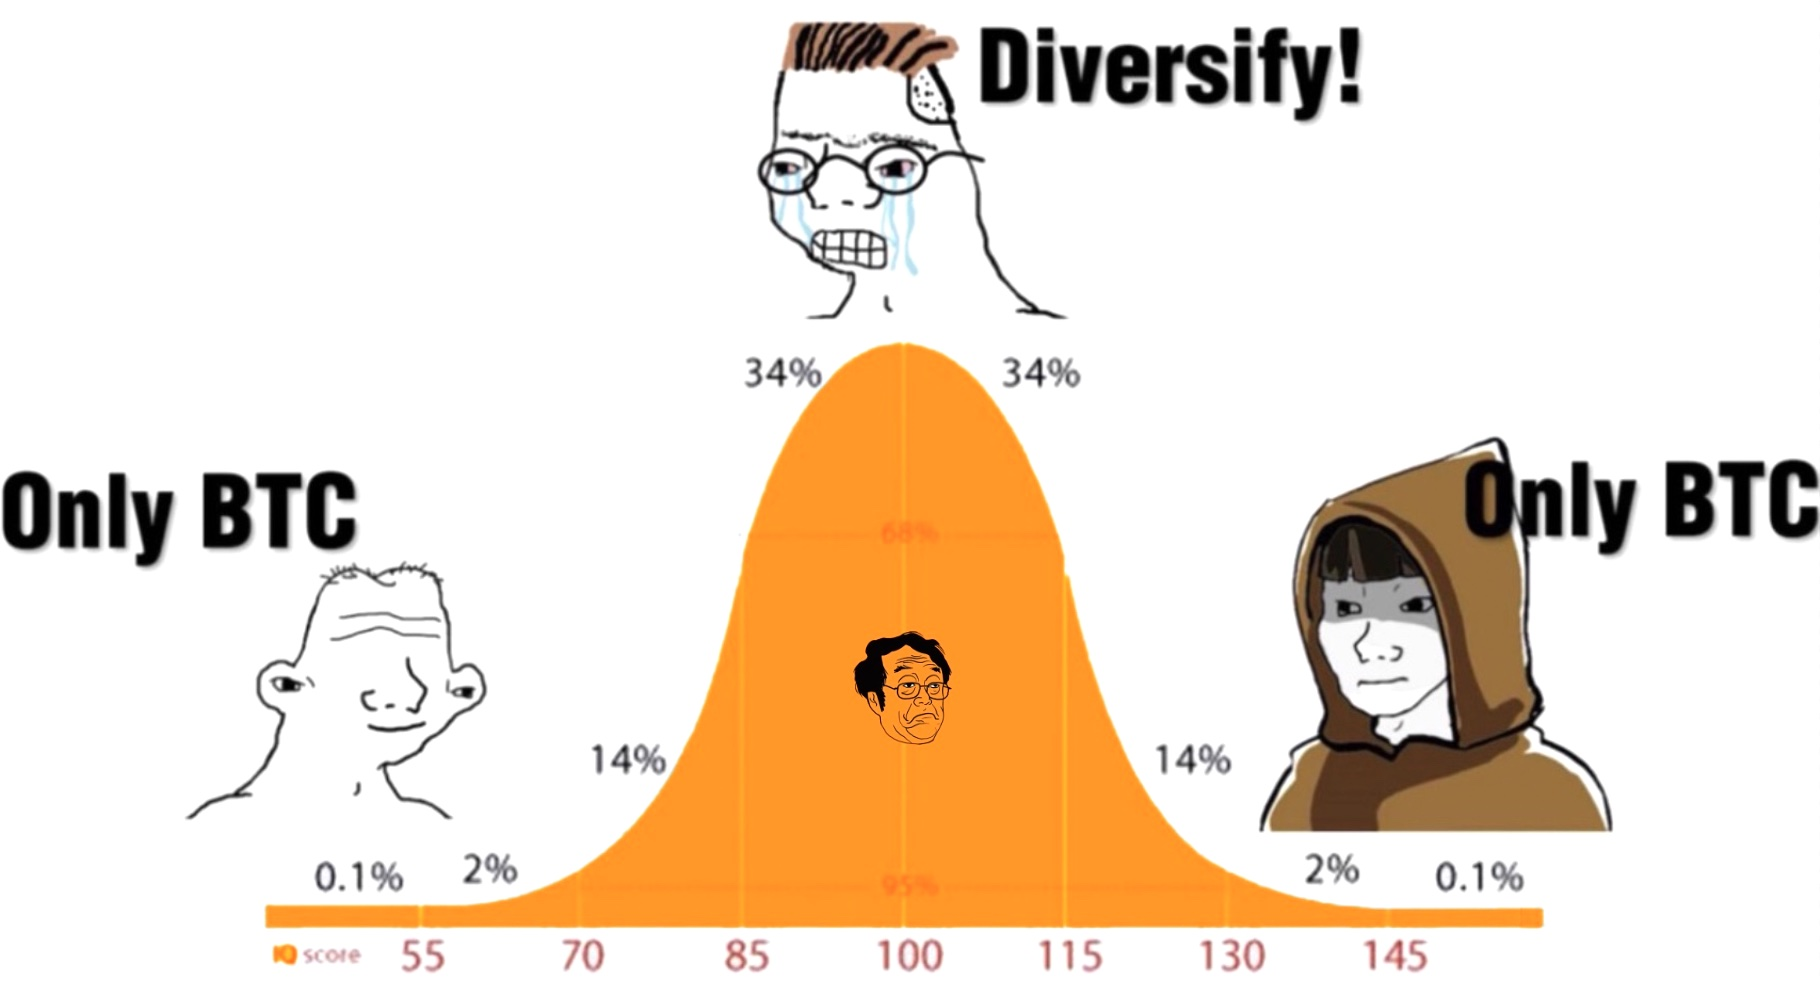
\includegraphics[keepaspectratio]{content/essentials/../../images/memes/bellcurve.jpg}}

}

\caption{BTC Bell Curve meme}

\end{figure}%

\section{Chad}\label{chad-1}

\begin{figure}[H]

{\centering \pandocbounded{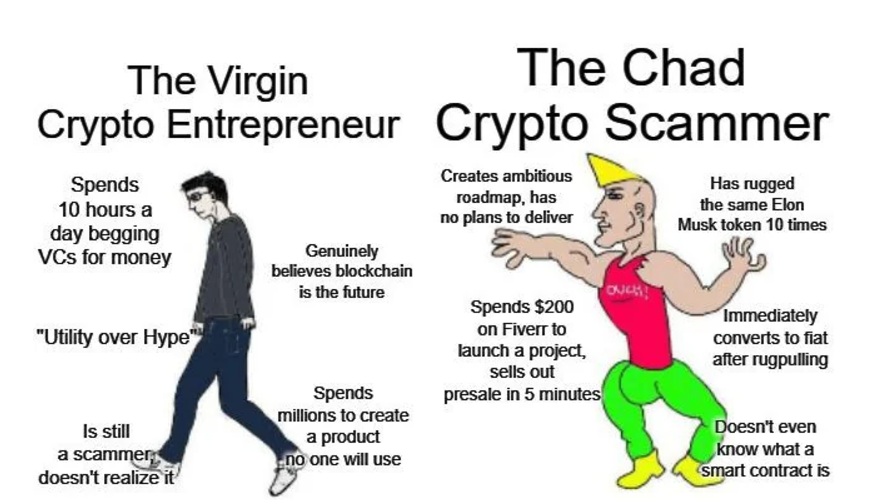
\includegraphics[keepaspectratio]{content/essentials/../../images/memes/chad.png}}

}

\caption{Chad}

\end{figure}%

\section{General}\label{general}

\begin{itemize}
\tightlist
\item
  Wojak/NPC: Originally from 4chan, this simple face drawing represents
  the average retail trader who buys high and sells low. It's often
  paired with the ``feels guy'' emotion variations, particularly during
  market crashes.
\item
  FUD (Fear, Uncertainty, Doubt): While not strictly a meme, it's become
  memefied in crypto culture. Any negative news or criticism is often
  dismissed as ``FUD'' by cryptocurrency enthusiasts, sometimes
  ironically.
\item
  ``When Lambo?'': This phrase emerged during the 2017 bull run,
  representing the dream of getting rich enough from crypto to buy a
  Lamborghini. It's both used seriously by newcomers and ironically by
  veterans.
\item
  Diamond Hands / Paper Hands: Popularized during the GameStop saga but
  heavily adopted in crypto. ``Diamond hands'' refers to holders who
  don't sell despite market pressure, while ``paper hands'' sell at the
  first sign of trouble.
\item
  ``This is good for Bitcoin'': Originally used seriously, it became
  ironic as people would claim any news, even negative, was somehow
  positive for Bitcoin's adoption or price.
\item
  Bogdanoff Twins (``Dump It''): These memes feature the late Bogdanoff
  twins supposedly controlling the crypto markets, ordering price dumps
  right after someone buys or pumps after they sell.
\item
  ``Funds are SAFU'': From a Binance CEO video where he mispronounced
  ``safe,'' this became a way to reassure (often ironically) about
  exchange security. The ``Have Fun Staying Poor'' (HFSP): Used by
  crypto enthusiasts towards skeptics, though it's increasingly used
  ironically, especially during bear markets. The DCA (Dollar Cost
  Average) Wojak: A calmer, more zen version of Wojak who simply buys
  regularly regardless of price, representing a more measured approach
  to investing.
\item
  ``Sir, this is a Wendy's'': Used when crypto discussions become overly
  technical or philosophical, reminding people not to take themselves
  too seriously.
\end{itemize}

\part{Become a Degen}

\chapter{Early stage Degen}\label{early-stage-degen}

\section{Purchasing your first
Crypto}\label{purchasing-your-first-crypto}

While as much as possible I'd like to respect and adhere to the ethos of
the early Cypherpunks, there's also the practicality of expecting
newcomers to be able to perform some of the advanced requirements that
are needed. So we'll take a pragmatic approach and introduce those
concepts in incremental levels of difficulty.

So the first thing anyone entering Web3 needs to do is to purcahse some
Crypto. In this Chapter we'll walk you through the process, with the
important caveats below:

\begin{itemize}
\tightlist
\item
  You'll need at least 6 US shit coins. Or in normie speak, \$5 US
  Dollars.
\end{itemize}

We will use Coinbase as the CEX for this section. You're more than
welcome to use your local CEX. For users in countries that don't have
access to CEX's, we'll detail how they can purchase their first crypto
with \href{https://bisq.network}{Bisq}.

Due to me wanting anyone to be able to get into crypto, I'm pretty
adamanant that it shouldn't cost more than \$5 for people to learn. This
is why I'd like to tailor this to start off with people purchasing ETH

https://bisq.network/downloads/

I'm using the Bisq 2 version, although at the time of writing, it's
still in beta. There is a minimum requirement of 6 USD. The median
income is approximately \$7 per day.

\begin{itemize}
\tightlist
\item
  The poorest 10\% of the world live on less than \$2 a day
\item
  About 50\% live on less thatn \$7 a day
\end{itemize}

On Bisq the minimum amount I could find someone willing to trade with me
is 10 USD. Also it's sold at a huge premium. Further disenfranchizing
the world's poor. As such if anyone wants to purchase Bitcoin for \$10
please reach out to me Bisq kinda sucks. Hodl Hodl looks like a much
better solution

Get them to create an account at a CEX. Explain KYC/AML

Talk about why you never hold funds on a CEX. Go through FTX, Mount Gox
and other failures. Then talk about wallets.

We're going with Phantom as it supports: * Bitcoin * Ethereum * Solana *
Base * Polygon

As of writing, TVL across Ethereum has 54\%, Solana 7\%, Base and
Bitcoin both \textasciitilde3\%. So while I'd love a wallet that
supports Stacks, Move and Cosmos. That just doesn't exist today. So as a
first time Web3 user, Phantom just makes the most sense. I also really
wanted users first wallet to have social recovery. But no wallet
currently supprots this. Argent used to, but they're now only on
Starknet and Soul wallet has no downloadable version I could find.

Need to talk about storing of private key

\begin{itemize}
\tightlist
\item
  Physical storage. These have a shit user experience, but are
  relatively safe. Hardware
\item
  Digital storage. Password manager, social recovery will come at some
  point
\end{itemize}

So we'll purchase ETH, transfer it to our Phantom wallet, and then stake
it on Lido

\section{Accounts}\label{accounts-1}

Here we'll go through Standard Accounts (EOA's) versus Smart Accounts.
Which blockchains support the different paradigms.

Issue with social recovery is that you leave a fingerprint to your on
chain activity depending on how the wallet handles the storing of your
data

The first place you're going to have to start is actually converting
fiat into crypto.

You can do this via:

\begin{itemize}
\tightlist
\item
  mining
\item
  purchasing
\end{itemize}

We'll only talk about purchasing here, as solo mining is not profitable,
although if you're not running at a loss, then it can still be
considered away of converting fiat into crypto.

\begin{itemize}
\tightlist
\item
  Privacy respecting ways

  \begin{itemize}
  \tightlist
  \item
    Peer to Peer (P2P) Marketplaces
  \item
    Bitcoin ATMs
  \end{itemize}
\item
  Non Privacy respecting ways

  \begin{itemize}
  \tightlist
  \item
    CEX's
  \item
    OTC
  \item
    DeFi on ramps
  \end{itemize}
\end{itemize}

For complete privacy, the place where you purchase

\chapter{Gigabrain Degen}\label{gigabrain-degen}

\section{Converting FIAT into a
Cryptocurrency}\label{converting-fiat-into-a-cryptocurrency}

This may be the hardest part of being a Degen. A Degen values privacy.
Important to distinguish there is a difference between privacy and
secrecy. I'd like my cryptocurrency to display the same characteristics
as cash. A means of exchange that has been working just fine for
centuries. Cash is private by default and people have seemed pretty
happy with that arrangement for over 3 centuries.

Currently the best way to do this is via:

\begin{itemize}
\tightlist
\item
  \href{https://bisq.network/}{Bisq}
\item
  \href{https://hodlhodl.com/}{HODL HODL}
\end{itemize}

\part{Financial}

\chapter{Digital Assets}\label{digital-assets}

The logical place to start this Almanack is Digital Assets. These
include all the financial instruments that exist within the Web3 sphere.
For us to represent all Digital Assets within this space, it means we
need to include all Web3 financial instruments, both on chain and off
chain.

We take inspiration from the
\href{https://www.usv.com/writing/2016/08/fat-protocols/}{Fat Protocol
Thesis}(Monegro 2016) to define the major categories of Digital Assets
within the Web3 realm. We also adhere to the naming convention that
stipulates Coins are digital assets relating to the running and
operation of a Blockchain, whereas Tokens are digital assets that are
issued on a Blockchain.

We thus break down Digital Assets into the following Categories:

\begin{itemize}
\tightlist
\item
  Coins

  \begin{itemize}
  \tightlist
  \item
    Primary Networks
  \item
    Secondary Networks

    \begin{itemize}
    \tightlist
    \item
      Ozempic
    \item
      Sugar
    \end{itemize}
  \item
    Derivatives
  \end{itemize}
\item
  Tokens

  \begin{itemize}
  \tightlist
  \item
    Fungibles
  \item
    Non Fungible
  \end{itemize}
\end{itemize}

After describing the various categories and classes of Digital Assets
we'll then delve into the Markets existing for these Digital Assets, as
well as how an entity \hyperref[hodl]{hodls} the Digital Asset and the
yield properties of the various types of Digital Assets.

\section{Coins}\label{coins}

This section deals primarily with Digital Assets as a Financial
Instrument and as such any information relating to the technical makeup
can be found in the \href{../technical/blockchains.qmd}{Blockchain}
documentation.

\subsection{Network Economics}\label{network-economics}

Token Models Utility Tokens: Gas fees, staking, governance Security
Tokens: Validator requirements, slashing deposits Network Tokens:
Transaction fees, block rewards Incentive Structures Validator Rewards:
Block rewards, transaction fees, staking yields User Incentives: Fee
markets, priority mechanisms, rebate systems Developer Incentives: Grant
programs, protocol fees, treasury funding Economic Security Minimum
Stakes: Validator requirements, delegation minimums Slashing Conditions:
Downtime penalties, malicious behavior penalties Market Making:
Liquidity incentives, trading pair support

\subsection{Base Networks}\label{base-networks}

This Almanack distinguishes between the financial properties of Coins
versus the technical properties of a
\href{../technical/blockchains.qmd}{Blockchain}. As such we don't refer
to networks here by Layer 1 or Layer 2. That's a classification and
distinction you can explore \hyperref[layer-1]{here}.

We define a Base Network that maintains it's own Sovereignity. This
means that the Coin on the network is used to economically secure the
chain as well as final settlement to occur on this network.

\subsection{Secondary Networks}\label{secondary-networks}

These are networks that market themselves as settling the transactions
on another network. The nuances of how they settle is covered under the
\href{../technical/blockchains.qmd}{Blockchain chapter}. We'll encompass
the full breadth of L2's including, but not limited to Plasma,
Sidechains, Rollups etc.

We then break these networks into Ozempic or Sugar networks. This
reflects a hat tip to the Fat protocol metaphor. Ozempic networks are
net extractors of value from their host chain, while Sugar networks
cause the host chain to become fatter and therefore hold more value.

Please see \hyperref[ozempic-effect]{Ozempic Effect} to see how we
determine if a network in a net ozempic or sugar network.

\subsection{Derivatives}\label{derivatives}

\begin{itemize}
\tightlist
\item
  On chain

  \begin{itemize}
  \tightlist
  \item
    Wrapped

    \begin{itemize}
    \tightlist
    \item
      Pure
    \item
      Bridged
    \end{itemize}
  \end{itemize}
\item
  Off Chain

  \begin{itemize}
  \tightlist
  \item
    Spot ETF's
  \end{itemize}
\end{itemize}

\subsubsection{On Chain Derivatives}\label{on-chain-derivatives}

\subsubsection{Off Chain Derivatives}\label{off-chain-derivatives}

\section{Tokens}\label{tokens}

\subsection{Fungible}\label{fungible}

Fungible is a pretty terrible name, but it roughly means divisable. It's
easier to explain via an example. If I have 10 dollars and I give you 3.
I still have 7. It's divisable. If I have a car and I want to give you
30\% of it, I cannot cut it up and give you a portion of it. It's Non
fungible, or non divisable. There's more nuances which we can deal with
in the vocabulary section. But that's the general idea of it.

We have the following types: * Stable Coins * Fiat backed * Crypto
backed * Delta Neutral backed * Shit Coins * Governance * Meme * Utility

Then we have numerous standards. We'll add only the most popular and
relevant ones here.

Namely: * ERC20 * ERC777 * ERC1363 * BRC20 * Runes * Solana's SPL Token
Standard * ICS20

\subsubsection{ICS20}\label{ics20}

The Inter-Chain Standard 20 is a \hyperref[cosmos-hub]{Cosmos} based
standard for fungible token transfers between blockchains using the
Inter-Blockchain Communication Protocol (IBC)

\subsection{Non Fungible}\label{non-fungible}

Has the following attributes:

\begin{itemize}
\tightlist
\item
  Art \& Collectibles
\item
  Profile Picture (PFP)
\item
  Gaming
\item
  Domain Names and Identity
\item
  Real World Assets (RWA)
\end{itemize}

The NFT floor price is the lowest price at which an NFT from a
particular collection is listed for sale on a marketplace. It serves as
a benchmark for the collection's market value and is widely used to
assess the entry point for potential buyers and to gauge the
collection's popularity and liquidity.

\section{Markets}\label{markets}

Where can I buy these Digital Assets? The major markets are regulated
and unregulated.

These are then divided into spot vs derivatives.

For regulated it's interesting as RedBelly in a blockchain, but it has
KYC/AML. So is that regularly compliant. It's probably more truthful to
break it down not by regulatory compliance, but anonymity. For if your
on chain activity can be tracked then most mature jurisdictions will be
able to force an individual to be compliant.

\section{Hodling}\label{hodling}

Wallets

\subsection{Custodial}\label{custodial}

\subsection{Non-Custodial}\label{non-custodial}

\begin{itemize}
\tightlist
\item
  Pure

  \begin{itemize}
  \tightlist
  \item
    Cold
  \item
    Hot
  \end{itemize}
\item
  Smart

  \begin{itemize}
  \tightlist
  \item
    MPC
  \item
    Smart Contract Based (Includes Account Abstraction)
  \end{itemize}
\end{itemize}

\section{Yield Properties}\label{yield-properties}

Major categories are:

\begin{itemize}
\tightlist
\item
  Network Yield
\item
  Trading Yield
\item
  Protocol Yield
\end{itemize}

\subsection{Trading Yield}\label{trading-yield}

\begin{itemize}
\tightlist
\item
  Pricing appreciation
\item
  Arbitrage Yield

  \begin{itemize}
  \tightlist
  \item
    Spot Arbitrage
  \item
    Peg Arbitrage - These are unique to stable coins
  \end{itemize}
\item
  Options and Derivatives Premiums
\item
  Futures funding rates
\end{itemize}

\subsection{Network Yield}\label{network-yield}

\begin{itemize}
\tightlist
\item
  Mining Yield

  \begin{itemize}
  \tightlist
  \item
    Solo Mining
  \item
    Pool Mining
  \item
    Cloud Mining
  \end{itemize}
\item
  Validating Yield

  \begin{itemize}
  \tightlist
  \item
    Staking
  \end{itemize}
\item
  Network Fee Yield

  \begin{itemize}
  \tightlist
  \item
    Gas
  \end{itemize}
\item
  MEV

  \begin{itemize}
  \tightlist
  \item
    Toxic
  \item
    Non Toxic
  \end{itemize}
\item
  Derivatives

  \begin{itemize}
  \tightlist
  \item
    Liquid Staking
  \end{itemize}
\end{itemize}

\subsection{dApp Yield}\label{dapp-yield}

\begin{itemize}
\tightlist
\item
  Staking
\item
  Liquidity Provision
\item
  Governance Participation
\item
  NFT Rental Income
\end{itemize}

\subsubsection{Liquidity Provision}\label{liquidity-provision}

We break this down into the following Categories

\begin{itemize}
\tightlist
\item
  AMM Pool fees
\item
  Concentrated liquidity positions
\item
  Order book market making
\item
  Lending and Borrowing markets
\end{itemize}

\paragraph{Concentrated Liquidity
Provision}\label{concentrated-liquidity-provision}

Here we will break down rebalancing and focus on Loss Versus Rebalancing
as per this paper https://arxiv.org/pdf/2208.06046

\chapter{Ratings}\label{ratings}

\section{Core Rating Categories (60\% of Total
Rating)}\label{core-rating-categories-60-of-total-rating}

\subsection{1. Protocol Value Capture
(30\%)}\label{protocol-value-capture-30}

A. Network Effect Metrics - Daily Active Users (DAUs) - Total Value
Locked (TVL) - Transaction volume - Fee revenue generated - Protocol
revenue retained

B. Value Accrual Mechanisms - Token economics design - Fee distribution
model - Staking mechanisms - Burns and supply dynamics

C. Ozempic Network Effects - Value extraction efficiency from L1 -
Transaction fee capture rate - User migration metrics from L1 - TVL
migration patterns - Gas savings versus L1 - L1-L2 Value Dynamics -
Sequencer revenue distribution - MEV capture and distribution - Bridge
volume and efficiency - Settlement layer costs - Sustainable Value
Creation - Net new users versus L1 migration - Ecosystem-specific
applications - Novel transaction types impossible on L1 - Cross-L2
interoperability metrics

\subsection{2. Protocol Security \& Risk Assessment
(30\%)}\label{protocol-security-risk-assessment-30}

A. Smart Contract Security - Audit history and quality - Bug bounty
program effectiveness - Historical vulnerability incidents - Code
complexity metrics - Upgrade mechanism security - Testing coverage

B. Network Security - Consensus mechanism robustness - MEV exposure and
protection measures - Node distribution - Network attack resistance -
Cross-chain bridge security - Oracle dependency and security

C. L1 Dependency Risks - Settlement layer congestion exposure - Bridge
security and liquidity depth - L1 fee market correlation - Sequencer
centralization risk - Value extraction sustainability

\section{Risk Categories (40\% of Total
Rating)}\label{risk-categories-40-of-total-rating}

\subsection{1. Technical Risk Assessment
(15\%)}\label{technical-risk-assessment-15}

A. Smart Contract Vulnerabilities - Code audit findings severity -
Time-tested deployment - Complexity of interactions - Dependencies on
external protocols - Historical incident analysis

B. Network Level Risks - MEV exposure metrics - Network partition
resistance - Node centralization factors - Infrastructure dependencies -
Cross-chain vulnerability exposure

C. Key Management \& Wallet Security - Multi-sig implementation - Key
generation processes - Hardware security modules usage - Social recovery
mechanisms - Access control systems

\subsection{2. Economic Risk Assessment
(10\%)}\label{economic-risk-assessment-10}

A. Market Dynamics - Liquidity concentration - Price impact resistance -
Collateral quality - Market manipulation resistance

B. Economic Model Vulnerabilities - Game theory attack vectors -
Incentive alignment analysis - Economic exploit resistance - Stress test
scenarios - Flash loan attack surface

\subsection{3. Operational Risk Assessment
(10\%)}\label{operational-risk-assessment-10}

A. CeFi/CeDeFi Risks - Centralization points - Custody arrangements -
Third-party dependencies - Operational redundancy - Emergency procedures

B. Oracle Dependencies - Oracle manipulation resistance - Price feed
reliability - Backup oracle systems - Historical oracle incidents - Data
quality metrics

\subsection{4. External Risk Assessment
(5\%)}\label{external-risk-assessment-5}

A. Regulatory Risk - Jurisdictional exposure - Compliance frameworks -
Regulatory clarity - Legal structure - Historical regulatory
interactions

B. Social Engineering Risk - Team security practices - Access control
policies - Social attack history - Security awareness training -
Incident response readiness

\section{Risk-Adjusted Rating Scale}\label{risk-adjusted-rating-scale}

AAA: Exceptional protocol with comprehensive risk mitigation - Multiple
independent security audits with no critical findings - Proven
resistance to all major attack vectors - Strong regulatory compliance
framework - Decentralized operations with minimal points of failure -
Multiple layers of economic security

AA: Strong protocol with robust risk management - Regular security
audits with minor findings - Documented resistance to common attack
vectors - Clear regulatory strategy - Limited centralization risks -
Strong economic security measures

\section{Risk Multipliers}\label{risk-multipliers}

Each risk category can apply a multiplier to the base rating: - Critical
Risk: -3 rating notches - High Risk: -2 rating notches - Medium Risk: -1
rating notch - Low Risk: No adjustment - Minimal Risk: +1 rating notch

\section{Continuous Monitoring
Triggers}\label{continuous-monitoring-triggers}

\begin{itemize}
\tightlist
\item
  Smart contract vulnerability disclosure
\item
  Network attack detection
\item
  Regulatory action
\item
  Economic model stress
\item
  Oracle deviation events
\item
  Cross-chain bridge incidents
\item
  Social engineering attempts
\item
  MEV activity spikes
\end{itemize}

\section{Review Framework}\label{review-framework}

\begin{itemize}
\tightlist
\item
  Monthly security metric review
\item
  Quarterly risk assessment update
\item
  Annual comprehensive review
\item
  Real-time monitoring of critical indicators
\item
  Incident-triggered reassessment
\end{itemize}

\section{Ozempic Effect}\label{ozempic-effect}

We'll base this upon value flows. Defillama doesn't actually display
this. So we'll need to get this data directly from the smart contracts.
We can start with Base, Arbitrum, BSC, Optimism and Polygon.

Let's build a comprehensive framework for tracking the true ``Ozempic
effect'' of L2s on Ethereum. We'll need several interconnected metrics
to understand the complete value flow dynamics.

\begin{enumerate}
\def\labelenumi{\arabic{enumi}.}
\tightlist
\item
  Wallet Migration Analysis
\end{enumerate}

\begin{itemize}
\tightlist
\item
  Track addresses that first appeared on Ethereum before a certain date
  (let's call them ``Ethereum Native Wallets'')
\item
  Monitor their activity transition to L2s over time
\item
  Analyze their ETH holdings distribution between L1 and L2s
\item
  Calculate the ratio of their transaction activity on L2s versus L1
\end{itemize}

\begin{enumerate}
\def\labelenumi{\arabic{enumi}.}
\setcounter{enumi}{1}
\tightlist
\item
  L2 Native User Analysis
\end{enumerate}

\begin{itemize}
\tightlist
\item
  Identify wallets that first appeared on L2s
\item
  Track what percentage never bridge to Ethereum
\item
  Measure their total value held
\item
  Calculate their transaction activity
\end{itemize}

\begin{enumerate}
\def\labelenumi{\arabic{enumi}.}
\setcounter{enumi}{2}
\tightlist
\item
  Fee Flow Dynamics
\end{enumerate}

\begin{itemize}
\tightlist
\item
  Track L2 sequencer fees paid back to Ethereum
\item
  Calculate the net fee difference (what these transactions would have
  cost on L1 versus actual L2 + L1 calldata costs)
\item
  Monitor the ratio of fees paid back to Ethereum versus fees retained
  by the L2
\end{itemize}

We could create a composite ``Value Migration Score'' that looks like:

\begin{Shaded}
\begin{Highlighting}[]
\KeywordTok{def}\NormalTok{ calculate\_migration\_score(l2\_data):}
    \CommentTok{\# Value Migration}
\NormalTok{    eth\_native\_migration }\OperatorTok{=}\NormalTok{ (}
\NormalTok{        eth\_native\_wallets\_on\_l2 }\OperatorTok{/}\NormalTok{ total\_eth\_native\_wallets }\OperatorTok{*}
\NormalTok{        eth\_value\_moved\_to\_l2 }\OperatorTok{/}\NormalTok{ original\_eth\_holdings}
\NormalTok{    )}
    
    \CommentTok{\# Activity Migration}
\NormalTok{    activity\_migration }\OperatorTok{=}\NormalTok{ (}
\NormalTok{        l2\_transactions\_by\_eth\_wallets }\OperatorTok{/} 
\NormalTok{        (l1\_transactions\_by\_eth\_wallets }\OperatorTok{+}\NormalTok{ l2\_transactions\_by\_eth\_wallets)}
\NormalTok{    )}
    
    \CommentTok{\# L2 Native Growth}
\NormalTok{    l2\_native\_strength }\OperatorTok{=}\NormalTok{ (}
\NormalTok{        l2\_only\_wallets }\OperatorTok{/}\NormalTok{ total\_l2\_wallets }\OperatorTok{*}
\NormalTok{        l2\_native\_value }\OperatorTok{/}\NormalTok{ total\_l2\_value}
\NormalTok{    )}
    
    \CommentTok{\# Fee Economics}
\NormalTok{    fee\_efficiency }\OperatorTok{=}\NormalTok{ (}
\NormalTok{        sequencer\_fees\_to\_ethereum }\OperatorTok{/} 
\NormalTok{        theoretical\_l1\_fees\_for\_same\_transactions}
\NormalTok{    )}
    
    \ControlFlowTok{return}\NormalTok{ (}
\NormalTok{        eth\_native\_migration }\OperatorTok{*} \FloatTok{0.3} \OperatorTok{+}
\NormalTok{        activity\_migration }\OperatorTok{*} \FloatTok{0.3} \OperatorTok{+}
\NormalTok{        l2\_native\_strength }\OperatorTok{*} \FloatTok{0.2} \OperatorTok{+}
\NormalTok{        fee\_efficiency }\OperatorTok{*} \FloatTok{0.2}
\NormalTok{    )}
\end{Highlighting}
\end{Shaded}

This would give us a quantitative measure of how effectively an L2 is:
1. Attracting value from Ethereum 2. Generating new value through native
users 3. Maintaining a sustainable fee relationship with Ethereum

A true Ozempic L2 should show: - High migration of ETH native wallets -
Strong L2 native user growth - Efficient fee generation that still
provides meaningful revenue to Ethereum - Sustained or growing activity
ratios over time

Would you like me to elaborate on how we could implement the data
collection for any of these metrics, or should we explore additional
factors to consider in the scoring?

\begin{itemize}
\tightlist
\item
  Net Value Extraction Rate = (Value Bridged In - Value Bridged Out) /
  Total Time Period
\end{itemize}

\section{Risk Factors}\label{risk-factors}

\subsection{1. Technical Risks}\label{technical-risks}

\begin{itemize}
\tightlist
\item
  Implementation bugs
\item
  Security vulnerabilities
\item
  Upgrade coordination failures
\item
  Network splits
\end{itemize}

\subsection{2. Governance Risks}\label{governance-risks}

\begin{itemize}
\tightlist
\item
  Capture by special interests
\item
  Low participation
\item
  Contentious decisions
\item
  Unclear processes
\end{itemize}

\subsection{3. Social Risks}\label{social-risks}

\begin{itemize}
\tightlist
\item
  Community fragmentation
\item
  Loss of developer support
\item
  Reputation damage
\item
  Market impacts
\end{itemize}

\section{Future Considerations}\label{future-considerations}

\subsection{1. Emerging Trends}\label{emerging-trends}

\begin{itemize}
\tightlist
\item
  Automated governance systems
\item
  AI-assisted proposal analysis
\item
  Cross-chain governance
\item
  Dynamic parameter adjustment
\end{itemize}

\subsection{2. Challenges}\label{challenges}

\begin{itemize}
\tightlist
\item
  Scaling governance participation
\item
  Balancing security and innovation
\item
  Managing increasing complexity
\item
  Maintaining decentralization
\end{itemize}

\subsection{3. Opportunities}\label{opportunities}

\begin{itemize}
\tightlist
\item
  Improved governance tools
\item
  Better simulation capabilities
\item
  Enhanced coordination mechanisms
\item
  More sophisticated voting systems
\end{itemize}

\section{Dependent Network Ratings}\label{dependent-network-ratings}

Polygon zkEVM Settlement Guarantees (10/10 weight): Score: 9/10 The
zkEVM uses zero-knowledge proofs to validate all state transitions.
Every transaction batch includes a proof that mathematically
demonstrates the correctness of all computations and state changes.
These proofs are verified by Ethereum's consensus mechanism, providing
cryptographic certainty that state transitions are valid. This is nearly
the highest level of settlement guarantee possible, just slightly below
fully integrated L2s because of some optimizations in the proving
system.

Dispute Resolution (9/10 weight): Score: 10/10 Ethereum serves as the
absolute source of truth for the zkEVM. If there's ever a dispute about
the state, the zero-knowledge proofs verified by Ethereum's consensus
provide mathematical certainty about what is correct. There's no
dependency on fraud proofs or challenge periods - the cryptographic
proofs mean disputes are resolved immediately and with absolute
certainty by Ethereum.

Economic Security Inheritance (8/10 weight): Score: 9/10 The zkEVM
inherits its fundamental security from Ethereum. The validity proofs
mean it can't confirm invalid state transitions, and its assets are
secured by Ethereum's consensus mechanism. While it has its own token
(MATIC) for gas fees and other purposes, the core economic security -
particularly for assets like ETH and tokens - comes directly from
Ethereum.

State Finality (7/10 weight): Score: 9/10 Once Ethereum confirms a zkEVM
batch and its validity proof, that state is final with the same
guarantees as Ethereum itself. The mathematical nature of the
zero-knowledge proofs means there's no waiting period for finality
beyond Ethereum's own finality period. This is as strong as state
finality can get for a settlement-dependent network.

Exit Rights Guarantees (6/10 weight): Score: 8/10 Users can always
withdraw their assets back to Ethereum by submitting a withdrawal
request. These withdrawals are guaranteed by Ethereum's consensus - once
a withdrawal is proven valid through a ZK proof, no one can prevent the
user from claiming their assets on Ethereum. The only limitation is the
normal proving and processing time.

State Progression Dependency (5/10 weight): Score: 7/10 While the zkEVM
can process transactions independently, it can't finalize new states
without submitting proofs to Ethereum and having them verified. This
creates a strong dependency on Ethereum for state progression, though
there's some independence in transaction processing.

Asset Movement (4/10 weight): Score: 10/10 Native ETH and ERC-20 tokens
can move seamlessly between Ethereum and the zkEVM. When assets move to
the zkEVM, they're locked on Ethereum and can only be unlocked through
valid proofs. This provides the strongest possible guarantees for asset
movement between the networks.

Total Score: 62/70 (approximately 89\%)

This analysis places Polygon zkEVM firmly in the ``Fully Non-Sovereign''
category. Arbitrum Let me analyze Arbitrum's relationship with Ethereum
as a Settlement-Dependent Network by carefully examining each criterion.
This will help us understand how optimistic rollups differ from ZK
rollups in their settlement dependency.

Settlement Guarantees (10/10 weight): Score: 7/10 Arbitrum uses an
optimistic rollup design where transactions are assumed valid but can be
challenged during a dispute period (currently 7 days). While this
provides strong settlement guarantees, it's not as immediate or
mathematically certain as ZK rollups. The challenge period introduces a
time-based element to settlement finality. However, the ability to prove
fraud on Ethereum's consensus layer still makes this a robust settlement
mechanism.

Dispute Resolution (9/10 weight): Score: 8/10 Ethereum serves as the
ultimate arbiter for Arbitrum through its fraud proof system. If someone
identifies an invalid state transition, they can submit a fraud proof to
Ethereum, which will automatically resolve the dispute and revert
invalid transactions. This is strong dispute resolution, though not as
immediate as ZK proofs since it requires active challengers and a
challenge period. The key strength is that Ethereum's consensus
automatically enforces the correct resolution once fraud is proven.

Economic Security Inheritance (8/10 weight): Score: 9/10 Arbitrum
inherits its fundamental security from Ethereum. The ability to prove
fraud on Ethereum means that any attempt to corrupt Arbitrum's state
would require corrupting Ethereum itself. The sequencer role adds some
centralization risk, but the fundamental economic security -
particularly for assets - comes directly from Ethereum. Users can always
force transactions through Ethereum if the sequencer fails.

State Finality (7/10 weight): Score: 6/10 While Arbitrum's state updates
are recorded on Ethereum, true finality requires waiting through the
challenge period. This creates a tradeoff between practical finality
(which can be quite fast) and absolute finality (which requires waiting
for the challenge period). This is lower than ZK rollups where finality
is immediate once proofs are verified.

Exit Rights Guarantees (6/10 weight): Score: 8/10 Users can always
withdraw their assets to Ethereum, guaranteed by Ethereum's consensus.
While withdrawals require waiting through the challenge period, they
cannot be prevented by Arbitrum's operators. The delay is longer than
with ZK rollups, but the guarantee is just as strong once the period
passes.

State Progression Dependency (5/10 weight): Score: 7/10 Arbitrum can
process transactions independently but must submit state roots to
Ethereum for potential verification. While it has more processing
independence than some systems, it ultimately depends on Ethereum for
final state confirmation, especially during disputes.

Asset Movement (4/10 weight): Score: 10/10 Native ETH and ERC-20 tokens
move seamlessly between Ethereum and Arbitrum through a strong bridge
mechanism backed by Ethereum's consensus. When assets move to Arbitrum,
they're locked on Ethereum and can only be unlocked through valid
withdrawals after the challenge period.

Total Score: 55/70 (approximately 79\%)

This analysis places Arbitrum in the ``Fully Non-Sovereign'' category,
though with a lower score than Polygon zkEVM. The main differences come
from the challenge period required for absolute finality and the
reliance on fraud proofs rather than validity proofs.

Stacks Settlement Guarantees (10/10 weight): Score: 4/10 Stacks uses
Bitcoin for checkpointing and security anchoring However, it lacks
cryptographic enforcement of settlement by Bitcoin's consensus Bitcoin
doesn't automatically enforce or validate Stacks' state transitions
Falls into the ``checkpoint systems'' category rather than stronger
settlement guarantees Dispute Resolution (9/10 weight): Score: 3/10
While Stacks records its state on Bitcoin, Bitcoin's consensus doesn't
serve as the ultimate arbiter Disputes are primarily resolved within
Stacks' own consensus mechanism Bitcoin can't automatically correct or
resolve issues in Stacks' state Economic Security Inheritance (8/10
weight): Score: 6/10 Miners must commit actual Bitcoin through PoX
mechanism This creates some economic security dependency on Bitcoin
However, Stacks maintains its own economic incentives through STX State
Finality (7/10 weight): Score: 5/10 Stacks achieves finality through a
combination of its own consensus and Bitcoin anchoring State is recorded
on Bitcoin but not in a way that Bitcoin consensus enforces Provides
stronger finality than fully independent chains but weaker than true L2s
Exit Rights Guarantees (6/10 weight): Score: 4/10 With sBTC, users can
move Bitcoin between chains However, this relies on Stacks' mechanisms
rather than being guaranteed by Bitcoin's consensus Exit rights depend
on threshold signatures rather than cryptographic guarantees State
Progression Dependency (5/10 weight): Score: 7/10 Stacks blocks are
linked to Bitcoin blocks through PoX State progression is tied to
Bitcoin's block progression However, Stacks can still process
transactions independently within this framework Asset Movement (4/10
weight): Score: 5/10 sBTC enables Bitcoin movement between chains But
this movement isn't directly enforced by Bitcoin's consensus Relies on
threshold signatures and Stacks' mechanisms Total Score: 34/59
(approximately 58\%)

This places Stacks in the ``Moderately Dependent'' category on our
spectrum.

\section{Risks}\label{risks}

Sub categories of risks include smart contract vulns regulatory risks
centralization risks for CeDeFi and CEX's MEV network level key and
wallet compromise cross chain exploits oracle manipulation Social
engineering exploitation of economic models Smart Contract Vulns Smart
contract vulnerabilities represent one of the most critical risks in
Web3, having led to billions in losses. This analysis examines major
exploit categories based on historical hacks, their prevalence across
different application models, and effective mitigation strategies.

Subcategories are: Access Control Flaws Logic and Arithmetic Errors
Oracle Manipulation Reentrancy attacks Flash Loan Vulnerabilities

Reentrancy attacks Mainly on Solidity. Famous example is the DAO hack
which resulted in the Ethereum. pre 0.4.0 of Solidity there were no
built in protections, so completely vulnerable.

Pre-0.4.0: No built-in protections, completely vulnerable 0.4.0-0.4.12:
Introduction of the transfer() function with 2300 gas stipend, providing
some protection but not comprehensive 0.4.13-0.7.x: Better compiler
warnings about state changes after external calls 0.8.0+: Enhanced
static analysis for potential reentrancy, but still requires explicit
protection

OpenZeppelin's ReentrancyGuard became the gold standard for protecting
against these attacks.

Move, used by Sui and Aptos, takes a different approach. It uses a
linear type system that treats resources as non-duplicatable assets.
This makes traditional reentrancy attacks much harder because resources
can't be accessed multiple times in the same transaction. However,
parallel execution in Sui could potentially create new forms of
reentrancy-like vulnerabilities.

High Risk (without additional protections): Solidity (EVM) - Requires
explicit guards and careful external call handling Medium Risk: Cairo
(StarkNet) - Possible but harder to accidentally create Cadence (Flow) -
Resource model helps but inter-contract calls need attention Low Risk
(by design): Move (Sui/Aptos) - Linear type system prevents traditional
reentrancy Rust (Solana) - Execution model prevents traditional
reentrancy Vyper (EVM) - Built-in restrictions prevent common reentrancy
patterns Clarity (Stacks) - Decidability and no recursive calls prevent
traditional reentrancy

\chapter{Trollip's Index}\label{trollips-index}

\section{Bitcoin}\label{bitcoin}

\section{Solana}\label{solana}

\section{Monero}\label{monero}

\section{Optimism}\label{optimism}

\section{Ethereum}\label{ethereum}

\section{Filecoin}\label{filecoin}

\section{Starknet}\label{starknet}

\section{Lido Staked Ethereum}\label{lido-staked-ethereum}

\section{Chainlink}\label{chainlink}

\section{Sui}\label{sui}

\section{Uniswap}\label{uniswap}

\section{Celestia}\label{celestia}

\section{XRP}\label{xrp}

\section{Dogecoin}\label{dogecoin}

\section{Tether USDT}\label{tether-usdt}

\section{Circle USDC}\label{circle-usdc}

\section{Ethena USDe}\label{ethena-usde}

\section{Aptos}\label{aptos}

\section{Arbitrum}\label{arbitrum}

\section{Stacks}\label{stacks}

\section{DAI}\label{dai}

\section{Cosmos Hub}\label{cosmos-hub}

\part{Technical}

\chapter{Cryptography}\label{cryptography}

\section{Symmetric Cryptography}\label{symmetric-cryptography}

Shared Keys. AES. But vulnerability is in sharing the Key between
parties.

\section{Asymetric Cryptography}\label{asymetric-cryptography}

Public Key Cryptography

RSA and elliptic curve cryptography. Slow than symetric cryptography.
Enables secure communication over insecure channels

\section{Hash functions}\label{hash-functions}

These are like digital fingerprints

\section{Zero-Knowledge Proofs}\label{zero-knowledge-proofs}

They solve a unique problem: how can you prove you know something
without revealing what you know? Imagine proving you're over 21 without
showing your actual birthdate.

\section{Homomorphic Encryption}\label{homomorphic-encryption}

It allows computations to be performed on encrypted data without
decrypting it first. Think of it like being able to ask someone to bake
a cake following your secret recipe, but without ever revealing the
recipe to them. While still computationally intensive, this technology
could revolutionize cloud computing and data privacy.

\section{Post-Quantum Cryptography}\label{post-quantum-cryptography}

cryptographic systems that can resist attacks from quantum computers.
This forward-looking field is essential because many current
cryptographic systems (especially asymmetric ones) could be broken by
powerful quantum computers.

\chapter{Blockchains}\label{blockchains-1}

We would prefer to use the term Decentralized Incentive Network instead
of blockchain. But we also want to align on common nomenclature within
the industry, so we'll stick with Blockchain for now.

The point of blockchains:

\begin{itemize}
\tightlist
\item
  Censorship resistance
\item
  Deterministic State Transition (Mempool creates interesting nuances
  and complexity here)
\item
  Credible neutrality
\item
  Trustless coordination at scale
\item
  Asset digitization and ownership
\end{itemize}

Censorship resistance is indeed crucial - it enables truly
permissionless systems where no entity can prevent valid transactions.
However, there are several other compelling candidates for blockchain's
primary purpose: One strong contender is deterministic state transition.
Think about how traditional databases or financial systems might have
ambiguity about the exact sequence or timing of transactions, especially
across different locations or institutions. Blockchain provides absolute
clarity about state changes - there's no ambiguity about which
transaction came first or what the exact state was at any given moment.
This property enables complex financial systems and smart contracts to
operate with complete predictability. Another fundamental purpose could
be creating credible neutrality in computational systems. This goes
beyond just censorship resistance - it's about creating systems where
the rules are explicit, unchangeable without consensus, and apply
equally to all participants. Traditional systems often have hidden
biases or special privileges for certain users, while blockchain systems
enforce their rules uniformly through code. We could also argue that the
primary purpose is enabling trustless coordination at scale. Before
blockchain, coordinating economic activity among untrusting parties
required trusted intermediaries like banks or governments. Blockchain
enables direct peer-to-peer coordination without these intermediaries,
potentially reducing costs and increasing efficiency. Asset digitization
and ownership might be another contender. Blockchain enables digital
scarcity and verifiable ownership in ways that weren't possible before.
This property enables everything from cryptocurrencies to NFTs to
tokenized real-world assets.

We won't be taking any idealogical approach to the point of blockchains
but rather applying scores to DIN's and then comparing that to how the
market values them.

A decentralized incentive network with state consensus

I've tried to simplify our definition as much as possible and even still
it's verbose. Read that sentence to 99\% of the world and I'll they'll
give you a quizzical look and move onto the section about meme coins.
There's a lesson there. A lesson the technical luminaries in this space
ignore at their peril. Accessibility matters.

Let's break down each component of our definition.

Decentralized. This is how many Nodes participate. Centralized means 1.
Therefore anything more than 1 is decentralized.

Network. This loosely means the participants computers/machines
communicate via a communication method.

State Consensus. The network will record state and all nodes will agree
about the state via consensus.

We don't need to worry too much about consensus yet, but you just need
to know that the nodes must agree on the state. For example if Bob sends
Alice 10 BTC. Everyone on the network must come to an agreement that Bob
did indeed send Alice 10 BTC. Another important characteristic is that
even if everyone agrees today, in the future that can't be disputed or
changed. This is another important category called censorship
resistance. We'll get to it.

Dependent Networks

A sovereign chain can be defined as a network that maintains complete
independence in its settlement process, requiring no external chain to
validate or guarantee its state transitions. This independence is
fundamental to the concept of sovereignty in blockchain networks.

This section should start discussing why the need arose for dependent
networks. Specifically Ethereum struggling with scale. Due to the
trilemna: decentralization security scalability

Let's talk about scaling strategies monolithic Bigger blocks Faster
blocks Higher minimum requirements for nodes Consensus optimizations
modular Execution - The current crop of L2's Data availability - Storing
and accessing blockchain data Celestia Consensus - Agreeing on the state
of the network Settlement - Finalizing transactions and providing
security guarantees. Ethereum and Bitcoin in the current Layer craze

\section{Sovereign Networks}\label{sovereign-networks}

Pure Value Networks Pure value networks stick to the fundamental purpose
of moving and storing value, avoiding the additional complexity that
comes with being a platform for applications or other services.

What makes these networks ``pure value'' is what they don't include:
They don't support complex smart contracts They don't host decentralized
applications They don't provide programmable functionality beyond basic
value transfer They don't serve as platforms for other tokens or
applications

Application Chains Application Chains represent networks that go beyond
pure value transfer to support various types of applications. They're
divided into three main categories: Hubs, Specialized, and Generalized
chains.

Hub Application Chains serve as central connection points in the
blockchain ecosystem.

Specialized Application Chains focus on specific use cases or
industries.

Generalized Application Chains aim to support a wide range of
applications but differ from hubs in that they're not necessarily trying
to be central connection points.

The key distinction between these categories lies in their approach to
applications: - Hubs prioritize becoming central platforms that other
networks depend on - Specialized chains optimize everything for specific
use cases - Generalized chains provide broad functionality but focus on
being self-contained ecosystems

\section{Layer 2's}\label{layer-2s}

We break these down into:

\begin{itemize}
\tightlist
\item
  Rollups

  \begin{itemize}
  \tightlist
  \item
    Optimistic
  \item
    ZK
  \end{itemize}
\item
  Validiums
\item
  Plasma
\item
  Sidechains
\end{itemize}

So Ethereum has chosen decentralization and security. This means
Ethereum is shit at scaling.

So we need to talk about the theory of Layers in Blockchain

That's why L2's became a major part of the roadmap. How does the
scalability limitation affect the network. Congestion and high gas
fee's. So people don't interact on the chain and it hits a ceiling. So
logically we should start any discussion with transaction fee's, as
that's the direct result of the scalability failure and the main reason
users use L2's. Besides yield opportunities.

So we should first consider the Fee Markets on Ethereum and Bitcoin
which are the two major chains looking to scale with L2's. There is a
lot of debate and a lot of misinformation around this topic.

Dependent networks can really be divided into chains: External DIN
required to validate state transitions External DIN required to
guarantee state transitions

We'll define a framework for how we define a Dependent Network. There
are few things we look at, in terms of priority: censorship resistance.
Polygon zkEVM sequencer can censure, but you can go through the contract
directly on Ethereum theoretically if censorship occurs. Same thing for
Arbitrum. Although this is a very weak guarantee due to the complexity
for regular users. For Stacks, it's more censorship resistant that the
other two. Also if I were to interact directly with the smart contract
on Ethereum, that makes the L2's pointless. Why do I need them if not to
deal with congestion and high gas. dispute resolution. I believe all
chains need to hard fork. Potentially not Movement due to Move's
resource model. None of the chains will automatically hard fork if a
dispute is found. settlement. So the base chain must validate and
guarantee state transitions on the dependent chain. This is kinda
stupid. It's guaranteeing the state transitions but makes no attempt to
resolve things like censorship resistance. finality of settlement.
Optimistic 7 days, zk 30 minutes, Stacks 16 hours economic security
model inheritance - this is actually pointless as it just means the
state transitions match the rules. Nothing about censorship resistance.

So my qualification of dependent networks means that they must inherit
the censorship resistance of the base chain, settlement must be
validated and guaranteed by the base chain, dispute resolution must be
automatic and/or decentralized. else the chain can just fork.

Settlement Types In order of strength Cryptographically enforced
settlement Validity proofs Fraud proof systems Checkpoint systems

Core Infrastructure Components Network Security Attack Vectors Network
Level: Eclipse attacks, BGP hijacking, DDoS attacks Protocol Level:
Double spending, nothing-at-stake, long-range attacks Application Level:
Smart contract vulnerabilities, oracle manipulation Defense Mechanisms
Network Diversity: Geographic distribution, client diversity, network
topology Economic Security: Slashing conditions, required stake amounts,
timelock mechanisms Operational Security: Key management, upgrade
processes, emergency responses Monitoring and Detection Network Health
Monitoring: Peer count, block propagation, chain quality Threat
Detection: Fork monitoring, unusual transaction patterns, validator
behavior Incident Response: Alert systems, mitigation procedures,
recovery processes Network Governance Governance Models On-Chain: Direct
token voting, delegated voting, quadratic voting Off-Chain:
Foundation-led, core team decisions, community forums Hybrid: Combined
on-chain execution with off-chain discussion Decision Domains Protocol
Parameters: Block size, gas limits, fee structures Treasury Management:
Fund allocation, grant distribution, development funding Protocol
Upgrades: Hard forks, soft forks, emergency changes Participation
Mechanisms Proposal Systems: Submission requirements, discussion
periods, voting periods Voting Methods: Token-weighted, identity-based,
reputation-based Execution Methods: Automatic execution, timelock
delays, manual implementation Cross-Chain Communication Bridge Types
Trusted Bridges: Custodial, multi-signature, federated Trustless
Bridges: Light clients, zero-knowledge proofs, relay networks Hybrid
Bridges: Combined trusted and trustless elements Message Passing
Protocol Standards: IBC (Inter-Blockchain Communication), cross-chain
messaging Verification Methods: SPV proofs, merkle proofs, validity
proofs Asset Standards: Wrapped tokens, synthetic assets, native bridges
Security Considerations Bridge Security: Validator sets, challenge
periods, fraud proofs Asset Security: Lockup mechanisms, minting
controls, burning procedures Network Security: Cross-chain replay
protection, nonce management

Network Performance Metrics Transaction Performance Throughput:
Transactions per second (TPS), block size limits Latency: Block time,
time to finality, confirmation time Costs: Transaction fees, gas costs,
execution costs Network Performance Block Propagation: Time to reach
network percentage Network Load: Memory pool size, peer connections,
bandwidth usage Chain Quality: Uncle rate, chain reorganizations, block
validity Resource Utilization Computing Resources: CPU usage, memory
requirements, storage growth Network Resources: Bandwidth consumption,
peer connections Storage Resources: State size, history size, pruning
capabilities Node Architecture Node Types Full Nodes: Complete state and
history validation Light Nodes: Header-only validation, SPV proofs
Archive Nodes: Complete historical state storage Validator Nodes: Block
production and validation Network Topology Peer Discovery: Bootstrap
nodes, DHT, static peers Connection Management: Maximum peers, scoring
systems, ban lists Data Propagation: Block propagation, transaction
propagation Resource Management State Management: State storage, pruning
policies, snapshot systems Network Management: Bandwidth limits, peer
limits, prioritization Computing Management: Transaction pools,
execution priorities Developer Infrastructure Development Tools SDKs:
Language support, library ecosystems, tool chains Testing Tools: Local
networks, test frameworks, simulation tools Monitoring Tools: Block
explorers, metrics, logging systems API Infrastructure RPC Endpoints:
JSON-RPC, GraphQL, WebSocket Node APIs: Client APIs, wallet interfaces,
indexer APIs Data Access: Block data, state data, historical data
Development Environment Local Development: Development networks, docker
environments Testing Networks: Test networks, faucets, explorers
Production Deployment: Network access, monitoring, maintenance

Common Concepts

State Growth \& Pruning Mechanisms Across Networks Ethereum State Growth
Unlimited state growth Historical state maintained by full nodes State
size \textasciitilde130GB and growing Uses Merkle Patricia Trie for
state storage Pruning Mechanisms Archive nodes store full history Full
nodes can prune historical states Light clients only store block headers
No protocol-level state expiry yet (proposed) Solana State Growth
Accounts model with rent mechanism State stored in memory for fast
access Accounts can be marked rent-exempt Program data separated from
account data Pruning Mechanisms Rent mechanism removes inactive accounts
Two years of inactivity leads to account cleanup Validators can prune
historical data Replicators store historical data Sui State Growth
Object-centric storage model Objects can be deleted explicitly Storage
fund for long-term costs Parallel execution reduces state bloat Pruning
Mechanisms Objects can be explicitly deleted Storage rebates incentivize
cleanup Validators can prune transaction history Maintains live object
set separately Aptos State Growth Account-based model Resources stored
under accounts Explicit resource deletion Storage fees for state growth
Pruning Mechanisms Storage fees incentivize cleanup Explicit resource
deletion Validators can prune historical states Maintains current state
tree XRP State Growth Account-based ledger Reserve requirements limit
state growth Objects can be deleted Amendable reserve requirements
Pruning Mechanisms Online deletion for historical data Reserve
requirements prevent spam Ledger header retention policy Configurable
history retention Stellar State Growth Account-based ledger Minimum
balance requirements Entry lifetime policies Base reserve adjustable by
voting Pruning Mechanisms Built-in entry expiration Configurable history
retention Minimum balance requirements Explicit deletion of unused
entries Polkadot State Growth Trie-based state storage Storage rent
(proposed) Bounded parachain growth Shared state across parachains
Pruning Mechanisms State rent mechanism (planned) Historical pruning
options Parachain state management Archive nodes for full history Layer
2 Solutions Optimistic Rollups (Optimism, Arbitrum) State growth tied to
L1 data availability Compression techniques for state updates Fraud
proof window affects state retention Can prune after challenge period ZK
Rollups (zkSync, StarkNet) State updates verified by ZK proofs More
efficient state representation Immediate finality enables pruning State
diffs published to L1 Key Patterns Growth Control MechanismsStorage
fees/rent Minimum balances Reserve requirements Explicit deletion
Pruning StrategiesHistorical pruning State expiry Account cleanup
Resource deletion Storage IncentivesRent mechanisms Storage rebates
Deletion incentives Reserve requirements

\section{Consensus Mechanisms}\label{consensus-mechanisms}

Consensus Mechanisms All DIN's have a consensus mechanism we have the
consensus mechanisms. These can be divided into the following broad
categories: Proof based mechanisms. Mainly Proof of Work and Proof of
Stake Byzantine Fault Tolerance (BFT) Mechanisms. Tendermint Voting
Based Mechanisms, Ripple and Stellar Directed Acrylic Graph based
mechanisms Hybrid. PoS + BFT is used by Polkadot and Cosmos Novel
Mechanisms

Need to talk about finality here about probabilistic vs deterministic.
Also focus on Single Slot Finality Proof-Based Mechanisms Proof of Work
(PoW) Security Model: Computational work as economic security Key
Properties: Energy-intensive computational puzzles Natural chain
selection through longest chain rule Strong resistance to Sybil attacks
High latency to finality Finality: Probabilistic finality with
increasing certainty over time Attack Resistance: 51\% attack requires
majority of network hashpower Very high cost of attack for established
networks Examples: Bitcoin, Ethereum (pre-merge), Litecoin Proof of
Stake (PoS) Security Model: Economic stake as security Key Properties:
Energy efficient Validator selection based on stake Slashing conditions
for misbehavior Lower latency than PoW Finality: Can achieve
deterministic finality with additional mechanisms Attack Resistance:
33\% or 51\% stake required depending on implementation Economic
penalties for malicious behavior Examples: Ethereum 2.0, Cardano, Tezos
Byzantine Fault Tolerance (BFT) Mechanisms Classical BFT Security Model:
Agreement among known validator set Key Properties: High throughput Low
latency Immediate finality Limited validator set size Finality: Instant
finality once consensus reached Attack Resistance: Tolerates up to 1/3
Byzantine validators Requires 2/3+ honest validators Examples:
Tendermint (Cosmos), Hyperledger Fabric Practical BFT (PBFT) Key
Properties: Three-phase commit protocol View change protocol for leader
failures Optimized for practical systems Performance Characteristics:
Higher message complexity Better performance in stable conditions
Examples: NEO, Hyperledger Sawtooth Voting-Based Mechanisms Federated
Byzantine Agreement (FBA) Security Model: Trust between validator groups
Key Properties: Quorum slices Flexible trust model Open validator set
Finality: Quick finality within trust boundaries Attack Resistance:
Based on trust overlap between validator groups Resistant to split votes
through quorum intersection Examples: Stellar, Ripple Delegated Proof of
Stake (DPoS) Security Model: Elected validator set Key Properties: Token
holder voting Limited validator set Regular validator rotation Finality:
Quick finality with selected validators Attack Resistance: Governance
attacks through voter collusion Validator collusion risks Examples: EOS,
TRON Directed Acyclic Graph (DAG) Based Pure DAG Security Model:
Transaction confirmation through subsequent references Key Properties:
Parallel transaction processing No explicit blocks Scalable throughput
Finality: Probabilistic with increasing certainty Attack Resistance:
Spam resistance through PoW Double-spend prevention through transaction
ordering Examples: IOTA, Hedera Hashgraph Block-DAG Security Model:
Hybrid of blockchain and DAG properties Key Properties: Multiple
concurrent blocks Complex ordering rules Higher throughput than linear
chains Examples: PHANTOM, SPECTRE Hybrid Mechanisms PoS + BFT Security
Model: Economic stake with BFT finality Key Properties: Stake-based
validator selection BFT consensus for finality Slashing for misbehavior
Finality: Deterministic through BFT layer Attack Resistance: Economic
security from stake Byzantine resistance from BFT Examples: Polkadot,
Cosmos PoW + BFT Security Model: Dual layer security Key Properties: PoW
for block production BFT for finality Higher security guarantees
Examples: Decred Novel Mechanisms Proof of History (PoH) Security Model:
Verifiable delay function for time ordering Key Properties: Built-in
timestamping Efficient verification High throughput Finality: Quick
finality with PoS integration Examples: Solana Avalanche Security Model:
Metastable consensus through repeated sampling Key Properties:
Sub-second finality High throughput Scalable validator set Finality:
Probabilistic with quick practical finality Examples: Avalanche Key
Considerations for Consensus Selection Performance Metrics Transaction
throughput Time to finality Network overhead Hardware requirements
Security Properties Byzantine fault tolerance Sybil resistance
Double-spend prevention Network partition handling Decentralization
Factors Validator set size Entry barriers Geographic distribution
Economic concentration Network Requirements Synchronicity assumptions
Bandwidth needs Storage requirements CPU/GPU demands Economic
Considerations Operating costs Required stake/investment Reward
distribution Slashing conditions

\section{Application Models}\label{application-models}

Add a section here on precompiled contracts All DIN's will have an
application model. So the Application model looks at the following:
state management parallelization Potential Asset Representation
Composability Safety Guarantees

UTXO also includes Cardano's extened UTXO, Kaspa also falls into this
Account Pure EVM, TRON Specialized XRP and Stelalr falls under this with
their balance-based model, Sharded account model Near falls into this.
Object (Sui) Aptos Resource model while different is moving towards an
Object model for Coins/Tokens Capability (Solana) Cell model (TON) Actor
Based (ICP and CosmWasm

\section{Communication Protocols}\label{communication-protocols}

We have

\begin{itemize}
\tightlist
\item
  IBC (Inter-Blockchain Communication) - Cosmos
\item
  XCMP (Cross-Chain Message Passing) - Polkadot
\item
  CCTP (Cross-Chain Transfer Protocol) by Circl
\item
  CCIP (Cross-Chain Interoperability) by Chainlink
\item
  Warp Messaging for Avalanche
\item
  IMP (Interchain Messaging Protocol)
\end{itemize}

We can then further classify these standard by the following properties:
* Security Model * Centralized vs Decentralized * Message Scope (General
(IBC,CCIP, Hyperlane) vs Specialized (Circle's CCTP and Warp)) * Open vs
Close networks * Message Verification Method

\section{Fee Markets}\label{fee-markets}

We break down fee markets into:

\begin{itemize}
\tightlist
\item
  Block Space Markets
\item
  Resources Markets
\end{itemize}

\subsection{Block Space Markets}\label{block-space-markets}

These are the most fundamental type. Users are paying for space in the
next block, regardless of what they're doing with that space. It only
considers the price of inclusion while respecting the limits of the
network.

\subsection{Resource Markets}\label{resource-markets}

These evolved with the advent of Ethereum as blockchains became more
complex. We break these down into:

\begin{itemize}
\tightlist
\item
  Compute
\item
  Data Availability
\item
  Storage
\item
  Hybrid
\end{itemize}

\subsubsection{Compute Markets}\label{compute-markets}

Transaction fee's sometimes called Gas is what you pay to execute a
smart contract on a blockchain. On some networks, like Ethereum, there
is an execution limit on how much computational work can be done in a
block. This parameter directly impacts the computational resources
required to run a node.

Nodes can propose a gas limit

So the attributes for Transactions Fee's are: Tips/Bribes How
Transactoin fees are distributed. Burnt or redirected to Miners How
fee's are calculated Base Fee Dynamic Fee (based on something like
network congestion)

\subsection{Data Availability}\label{data-availability}

We will compare the mechanisms of the following major DA layers:

\begin{itemize}
\tightlist
\item
  Ethereum
\item
  Celestia
\item
  Eignlayer DA
\item
  Avail
\end{itemize}

Ethereum uses dynamic blob fees based upon a target amount of blob space
per block.

Celestia charges by size. Celestia is designed to scale to handle
increase demand with adding more validators

Avail also charges by size but also the type.

EigenDA creates a marketplace for data availability providers

\subsubsection{Storage}\label{storage}

\subsubsection{Hybrid}\label{hybrid}

\subsubsection{Congestion Measurement
Mechanisms}\label{congestion-measurement-mechanisms}

\textbf{Ethereum}

\begin{itemize}
\tightlist
\item
  Measures block gas utilization vs 15M target
\item
  12.5\% base fee adjustment per block
\item
  Block size can flex up to 30M gas
\end{itemize}

\textbf{Stellar}

\begin{itemize}
\tightlist
\item
  Uses surge pricing mechanism
\item
  Triggers when ledger capacity exceeds 50\%
\item
  Fee increases proportionally to network load
\end{itemize}

\textbf{Polkadot}

\begin{itemize}
\tightlist
\item
  Uses weight-based system
\item
  Measures block weight against target
\item
  Adjusts fees based on block fullness
\end{itemize}

\textbf{Tezos}

\begin{itemize}
\tightlist
\item
  Monitors block saturation
\item
  Adjusts fees based on recent block usage
\item
  Uses gas limits per operation type
\end{itemize}

\subsection{Data Availability market}\label{data-availability-market}

Ethereum uses blobs, which are special containers for Layer 2 rollups to
post their transaction data. They also disappear after a time.

Blob fee is calculated based on the target blob gas per block.

\section{Network Change Management}\label{network-change-management}

\subsection{Overview}\label{overview}

Network change management in DINs encompasses the processes, mechanisms,
and stakeholders involved in proposing, discussing, approving, and
implementing network modifications. This framework covers everything
from minor parameter adjustments to major protocol upgrades.

\textbf{TODO} Design something that can simulate

\section{Clients}\label{clients}

\section{Bridges}\label{bridges}

Classification of Bridges. Need to include Lazy Bridges here
https://blog.celestia.org/lazybridging/

\begin{itemize}
\tightlist
\item
  Trusted

  \begin{itemize}
  \tightlist
  \item
    Custodial
  \item
    Multi Signature
  \item
    Federated
  \end{itemize}
\item
  Trustless Bridges

  \begin{itemize}
  \tightlist
  \item
    Light Client
  \item
    ZK

    \begin{itemize}
    \tightlist
    \item
      Lazy Bridge
    \end{itemize}
  \item
    Relay
  \end{itemize}
\end{itemize}

\chapter{dApps}\label{dapps}

dApps can be single chain or multichain. However they must exist on a
DIN and can't exist independently from a DIN. They don't need to have a
token to be included here. If an NFT develops functionality, they
they'll be inlcuded here too. They can be DeFi SocialFi GameFi CeDeFi
Concepts Concepts Flash loans DeFi Derivatives Basis Trading DEX Lending
Utility Yield Pendle 3k in Basis Trading Current dApps Ethena USDX
BounceBit

Derivatives Liquid staking Derivatives such as Lido, and EtherFi is the
primary element here Lending

SocialFi Meme Coins CeDeFi Circle fits in here GameFi

\chapter{MEV}\label{mev}

\section{Proposer Builder Separation
(PBS)}\label{proposer-builder-separation-pbs}

\section{Multiple Concurrent Leaders}\label{multiple-concurrent-leaders}

https://x.com/aeyakovenko/status/1810222589991583922

\part{Social}

\chapter{Governance}\label{governance}

This section will compare how Blockchains implement the three tiers of
traditional governance. Namely:

\begin{itemize}
\tightlist
\item
  Legistlative - Who makes the rules and how they created
\item
  Executive - Who executes the rules
\item
  Judicial - Referee between them
\end{itemize}

So in Bitcoin BIP's cover the Legislative aspect, Executive is Node
operators for Networks then for dapps it gets more complex. Judicial is
where it gets challenging. This is pretty much the entire community.
People interpret rules by economic activity and nodes. Look at Bitcoin
Cash. No money. So everyone agreed with the block size of Bitcoin.

There is also the concept of Canvassing or Lobbying can also occur.
Let's look at Ethereum. If I wanted to increase the gas limit from 30
million to 31 million. I'd need to canvas all the nodes to come along
with me. Currently there is 5,333 nodes. So I'd need to convince
\textasciitilde3k node operators to increase the gas limit.

\subsubsection{1. Hard Forks}\label{hard-forks}

\begin{itemize}
\tightlist
\item
  \textbf{Definition}: Protocol changes that make previously invalid
  blocks/transactions valid (or vice-versa), requiring all nodes to
  upgrade
\item
  \textbf{Characteristics}:

  \begin{itemize}
  \tightlist
  \item
    Non-backwards compatible
  \item
    Requires coordinated network upgrade
  \item
    Creates potential for chain splits if not unanimously adopted
  \end{itemize}
\item
  \textbf{Use Cases}: Major protocol upgrades, fundamental rule changes,
  bug fixes
\item
  \textbf{Examples}: Ethereum's merge to PoS, Bitcoin's SegWit upgrade
\end{itemize}

\subsubsection{2. Soft Forks}\label{soft-forks}

\begin{itemize}
\tightlist
\item
  \textbf{Definition}: Backwards-compatible protocol changes that
  tighten rules without invalidating existing blocks
\item
  \textbf{Characteristics}:

  \begin{itemize}
  \tightlist
  \item
    Backwards compatible
  \item
    Old nodes can still participate (with limitations)
  \item
    Lower coordination requirements
  \end{itemize}
\item
  \textbf{Use Cases}: Adding new features, incremental improvements
\item
  \textbf{Examples}: Bitcoin's P2SH implementation, taproot upgrade
\end{itemize}

\subsubsection{3. Parameter Updates}\label{parameter-updates}

\begin{itemize}
\tightlist
\item
  \textbf{Definition}: Changes to network variables within predefined
  bounds
\item
  \textbf{Characteristics}:

  \begin{itemize}
  \tightlist
  \item
    No code changes required
  \item
    Often automated through on-chain governance
  \item
    Lower risk than protocol changes
  \end{itemize}
\item
  \textbf{Use Cases}: Fee adjustments, block size modifications, staking
  parameters
\item
  \textbf{Examples}: Tezos' regular parameter updates, Cosmos'
  governance parameters
\end{itemize}

\subsection{Governance Mechanisms}\label{governance-mechanisms}

\subsubsection{1. Off-Chain Governance}\label{off-chain-governance}

\begin{itemize}
\tightlist
\item
  \textbf{Characteristics}:

  \begin{itemize}
  \tightlist
  \item
    Social consensus through discussion forums, social media,
    conferences
  \item
    Informal decision-making processes
  \item
    Relies on node operator coordination
  \end{itemize}
\item
  \textbf{Advantages}:

  \begin{itemize}
  \tightlist
  \item
    Flexible and adaptable
  \item
    Allows for nuanced discussion
  \item
    Natural resistance to capture
  \end{itemize}
\item
  \textbf{Disadvantages}:

  \begin{itemize}
  \tightlist
  \item
    Can be slow and messy
  \item
    May lack clear resolution mechanisms
  \item
    Potential for contentious outcomes
  \end{itemize}
\end{itemize}

\subsubsection{2. On-Chain Governance}\label{on-chain-governance}

\begin{itemize}
\tightlist
\item
  \textbf{Characteristics}:

  \begin{itemize}
  \tightlist
  \item
    Formal voting mechanisms
  \item
    Smart contract-based execution
  \item
    Token-weighted or identity-based participation
  \end{itemize}
\item
  \textbf{Advantages}:

  \begin{itemize}
  \tightlist
  \item
    Clear process and outcomes
  \item
    Automated execution
  \item
    Transparent participation
  \end{itemize}
\item
  \textbf{Disadvantages}:

  \begin{itemize}
  \tightlist
  \item
    Potential plutocratic capture
  \item
    Reduced flexibility
  \item
    Voter apathy risks
  \end{itemize}
\end{itemize}

\subsubsection{3. Hybrid Systems}\label{hybrid-systems}

\begin{itemize}
\tightlist
\item
  \textbf{Characteristics}:

  \begin{itemize}
  \tightlist
  \item
    Combines off-chain discussion with on-chain execution
  \item
    Multiple stages of proposal refinement
  \item
    Mixed participation models
  \end{itemize}
\item
  \textbf{Advantages}:

  \begin{itemize}
  \tightlist
  \item
    Balances flexibility with formality
  \item
    Combines benefits of both approaches
  \item
    Can adapt to different types of changes
  \end{itemize}
\item
  \textbf{Examples}: Polkadot's governance system, Cosmos Hub's proposal
  process
\end{itemize}

\subsection{Improvement Proposal
Systems}\label{improvement-proposal-systems}

\subsubsection{1. Structure}\label{structure}

\begin{itemize}
\tightlist
\item
  \textbf{Stages}:

  \begin{itemize}
  \tightlist
  \item
    Draft: Initial proposal development
  \item
    Review: Community feedback and refinement
  \item
    Last Call: Final period for major objections
  \item
    Accepted/Final: Ready for implementation
  \item
    Rejected: Proposal declined
  \end{itemize}
\item
  \textbf{Components}:

  \begin{itemize}
  \tightlist
  \item
    Technical specification
  \item
    Motivation and rationale
  \item
    Backwards compatibility analysis
  \item
    Reference implementation (if applicable)
  \item
    Security considerations
  \end{itemize}
\end{itemize}

\subsubsection{2. Common Frameworks}\label{common-frameworks}

\begin{itemize}
\tightlist
\item
  \textbf{BIP (Bitcoin Improvement Proposals)}:

  \begin{itemize}
  \tightlist
  \item
    Focus on consensus changes
  \item
    Conservative approach
  \item
    High emphasis on security
  \end{itemize}
\item
  \textbf{EIP (Ethereum Improvement Proposals)}:

  \begin{itemize}
  \tightlist
  \item
    Multiple tracks (Core, ERC, Interface)
  \item
    Regular cadence of updates
  \item
    Strong emphasis on standardization
  \end{itemize}
\item
  \textbf{Network-Specific Systems}:

  \begin{itemize}
  \tightlist
  \item
    Customized to network needs
  \item
    Varying levels of formality
  \item
    Different voting thresholds
  \end{itemize}
\end{itemize}

\subsection{Centralization Factors}\label{centralization-factors}

\subsubsection{1. Development
Centralization}\label{development-centralization}

\begin{itemize}
\tightlist
\item
  \textbf{Core Development Teams}:

  \begin{itemize}
  \tightlist
  \item
    Control over codebase
  \item
    Technical expertise concentration
  \item
    Funding dependencies
  \end{itemize}
\item
  \textbf{Client Implementation}:

  \begin{itemize}
  \tightlist
  \item
    Diversity of node software
  \item
    Implementation independence
  \item
    Bug discovery and fixes
  \end{itemize}
\end{itemize}

\subsubsection{2. Governance
Centralization}\label{governance-centralization}

\begin{itemize}
\tightlist
\item
  \textbf{Voting Power Distribution}:

  \begin{itemize}
  \tightlist
  \item
    Token concentration
  \item
    Delegate systems
  \item
    Voter participation rates
  \end{itemize}
\item
  \textbf{Proposal Control}:

  \begin{itemize}
  \tightlist
  \item
    Who can propose changes
  \item
    Filtering mechanisms
  \item
    Discussion venue control
  \end{itemize}
\end{itemize}

\subsubsection{3. Infrastructure
Centralization}\label{infrastructure-centralization}

\begin{itemize}
\tightlist
\item
  \textbf{Node Operation}:

  \begin{itemize}
  \tightlist
  \item
    Geographic distribution
  \item
    Hardware requirements
  \item
    Operating costs
  \end{itemize}
\item
  \textbf{Service Providers}:

  \begin{itemize}
  \tightlist
  \item
    API services
  \item
    Block explorers
  \item
    Development tools
  \end{itemize}
\end{itemize}

\subsection{Best Practices}\label{best-practices}

\subsubsection{1. Change Management}\label{change-management}

\begin{itemize}
\tightlist
\item
  Clear documentation of changes
\item
  Adequate testing periods
\item
  Coordinated upgrade schedules
\item
  Emergency response procedures
\end{itemize}

\subsubsection{2. Community Engagement}\label{community-engagement}

\begin{itemize}
\tightlist
\item
  Regular communication channels
\item
  Multiple feedback mechanisms
\item
  Transparent decision-making
\item
  Educational resources
\end{itemize}

\subsubsection{3. Technical
Implementation}\label{technical-implementation}

\begin{itemize}
\tightlist
\item
  Comprehensive testing frameworks
\item
  Clear upgrade paths
\item
  Fallback mechanisms
\item
  Security audits
\end{itemize}

\bookmarksetup{startatroot}

\chapter{Contributing}\label{contributing}

Here we'll list all the outstanding contributions we're looking for.

\bookmarksetup{startatroot}

\chapter*{References}\label{references}
\addcontentsline{toc}{chapter}{References}

\markboth{References}{References}

\phantomsection\label{refs}
\begin{CSLReferences}{1}{0}
\bibitem[\citeproctext]{ref-buterin2013ethereum}
Buterin, Vitalik. 2013. {``Ethereum White Paper: A Next Generation Smart
Contract \& Decentralized Application Platform.''}
\url{https://ethereum.org/en/whitepaper/}.

\bibitem[\citeproctext]{ref-buterin2021rollups}
---------. 2021. {``An Incomplete Guide to Rollups.''}
\url{https://vitalik.ca/general/2021/01/05/rollup.html}.

\bibitem[\citeproctext]{ref-charbonneau2023rollups}
Charbonneau, Jon. 2023. {``The Complete Guide to Rollups.''} Research
Report. Delphi Digital.
\url{https://members.delphidigital.io/reports/the-complete-guide-to-rollups}.

\bibitem[\citeproctext]{ref-dibona1999open}
DiBona, Chris, Sam Ockman, and Mark Stone. 1999. \emph{Open Sources:
Voices from the Open Source Revolution}. Sebastopol, CA: O'Reilly Media.

\bibitem[\citeproctext]{ref-gluchowski2021zkrollup}
Gluchowski, Alex. 2019. {``zkRollup Vs. Optimistic Rollup: Technical
Comparison.''} Matter Labs.
\url{https://medium.com/matter-labs/zkrollup-vs-optimistic-rollup-deep-dive-ea141e71e075}.

\bibitem[\citeproctext]{ref-hughes1993cypherpunk}
Hughes, Eric. 1993. {``A Cypherpunk's Manifesto,''} March.
\url{https://www.activism.net/cypherpunk/manifesto.html}.

\bibitem[\citeproctext]{ref-may1988cryptoanarchist}
May, Timothy C. 1988. {``The Crypto Anarchist Manifesto.''}
\url{https://www.activism.net/cypherpunk/crypto-anarchy.html}.

\bibitem[\citeproctext]{ref-monegro2016fat}
Monegro, Joel. 2016. {``Fat Protocols.''} Union Square Ventures.
\url{https://www.usv.com/writing/2016/08/fat-protocols/}.

\bibitem[\citeproctext]{ref-nakamoto2008bitcoin}
Nakamoto, Satoshi. 2008. {``Bitcoin: A Peer-to-Peer Electronic Cash
System.''} \url{https://bitcoin.org/bitcoin.pdf}.

\bibitem[\citeproctext]{ref-poon2017plasma}
Poon, Joseph, and Vitalik Buterin. 2017. {``Plasma: Scalable Autonomous
Smart Contracts.''} \url{https://plasma.io/plasma-whitepaper.pdf}.

\bibitem[\citeproctext]{ref-poon2016lightning}
Poon, Joseph, and Thaddeus Dryja. 2016. {``The Bitcoin Lightning
Network: Scalable Off-Chain Instant Payments.''}
\url{https://lightning.network/lightning-network-paper.pdf}.

\end{CSLReferences}




\end{document}
